\documentclass[12pt,titlepage]{article}
\usepackage{wrapfig}
\usepackage{svg}
\usepackage{nomencl}
\usepackage[american]{babel}
\usepackage[utf8]{inputenc}
\usepackage[T1]{fontenc}
\usepackage{lmodern}
\usepackage{amsmath,amsfonts,amssymb}
\usepackage{graphicx}
\usepackage{geometry}
\geometry{a4paper}
\usepackage[parfill]{parskip}
\usepackage{amssymb}

\usepackage{color}
\usepackage[tt]{titlepic}
\usepackage{fancyhdr}
\usepackage{enumerate}
\usepackage{lastpage}
\usepackage{bm}

\usepackage{listings}
\usepackage{tcolorbox}
\definecolor{codegreen}{rgb}{0,0.6,0}
\definecolor{codegray}{rgb}{0.5,0.5,0.5}
\definecolor{codepurple}{rgb}{0.58,0,0.82}
\definecolor{backcolour}{rgb}{0.95,0.95,0.92}
 
\lstdefinestyle{mystyle}{
    backgroundcolor=\color{backcolour},   
    commentstyle=\color{codegreen},
    keywordstyle=\color{magenta},
    numberstyle=\tiny\color{codegray},
    stringstyle=\color{codepurple},
    basicstyle=\footnotesize,
    breakatwhitespace=false,         
    breaklines=true,                 
    captionpos=b,                    
    keepspaces=true,                 
    numbers=left,                    
    numbersep=5pt,                  
    showspaces=false,                
    showstringspaces=false,
    showtabs=false,                  
    tabsize=2
}
 
\lstset{style=mystyle}

\usepackage[section]{placeins}
\usepackage{amsfonts}
\usepackage{amsmath}
\usepackage{float}
\usepackage{setspace}
\usepackage[justification=raggedright]{caption}
\usepackage{sidecap}

\usepackage{xcolor}
\usepackage{framed}
\definecolor{shadecolor}{RGB}{240,240,240}


\usepackage{booktabs}
\usepackage{multirow}

\usepackage[squaren, Gray, cdot]{SIunits}
\graphicspath{{image/}} %chemin par défaut pour aller chercher les images 
\usepackage{url}
\usepackage[utf8]{inputenc}
% FOR DEFINITIONS (https://www.sharelatex.com/learn/Theorems_and_proofs)
\usepackage{amsthm}
\theoremstyle{plain}
\newtheorem{definition}{Definition}[section]
\newtheorem*{definition*}{Definition}
\newtheorem{prop}{Proposition}
\newtheorem*{prop*}{Proposition}
\theoremstyle{remark}
\newtheorem*{remark}{Remark}
\newtheorem*{corollary}{Corollary}
\newtheorem{theorem}{Theorem}[section]
\newtheorem{lemma}[theorem]{Lemma}
\newtheorem*{example}{Example}
\usepackage{afterpage}

\newcommand\blankpage{
\null
\thispagestyle{empty}
\newpage}

% Custom Defines
\usepackage[comma,numbers,sort&compress]{natbib}
\bibliographystyle{plainnat}
\usepackage[pdfstartview=FitH,
            breaklinks=true,
            bookmarksopen=true,
            bookmarksnumbered=true,
            colorlinks=true,
            linkcolor=black,
            citecolor=black
            ]{hyperref}
\newcommand{\rmd}{\textrm{d}}
\newcommand{\norm}[1]{\left\lVert#1\right\rVert}
\newcommand{\bi}[1]{{\ensuremath{\boldsymbol{#1}}}}
\definecolor{gray}{rgb}{0.5,0.5,0.5}

\topmargin=-0.45in      %
%\evensidemargin=0in     %
\oddsidemargin=+0.5in      %
\textwidth=5.5in        %
\textheight=9.2in       %
%\headsep=0.25in         %
\headheight=30.9pt
\linespread{1.3}

\begin{document}

% ========== TITLE PAGE ===================================================
%!TEX root = 0.main.tex

\begin{titlepage}
\newcommand{\HRule}{\rule{\linewidth}{1mm}} % Defines a new command for the horizontal lines, change thickness here
\begin{minipage}[t]{.49\textwidth}
	\raggedleft
	\center
	\textsc{\footnotesize Politecnico di Milano}\\
	\textsc{ \scriptsize School of Industrial and Information Engineering}\\
	\textsc{\scriptsize Department of Mathematics}\\[0.5cm]
	
\includegraphics[width=5cm]{figs/cover/polimi.png}
\end{minipage}
\hfill
%
\begin{minipage}[t]{.49\textwidth}
	\raggedright
	\center
	\textsc{\footnotesize \'Ecole Polytechnique F\'ed\'erale de Lausanne}\\
	\textsc{\scriptsize School of Basic Sciences}\\
	\textsc{\scriptsize Department of Mathematics}\\[0.8cm]
	
\includegraphics[width=5cm]{figs/cover/EPFL.jpg}
\end{minipage}
\center % Center everything on the page
\vspace{2cm}





%	HEADING SECTIONS
\textsc{\large Master Thesis in Computational Science and Engineering}\\[1.5cm]

%	TITLE SECTION
\HRule \\[0.4cm]
{ \LARGE \bfseries About the spectrum of the Discrete Laplace-Beltrami operator on the Sphere for Rotation Equivariant Neural Networks}\\[0.4cm] 
\HRule \\[1.5cm]     
\vfill 
%	AUTHOR SECTION

\begin{minipage}{1\textwidth}
	\begin{flushleft} \large
		Supervisors: \hspace{0.3cm} Micha\"el Defferrard\\
		\hspace{3.2cm} prof. Piercesare Secchi\\
		\hspace{3.2cm} prof. Pierre Vandergheynst\\
		Co-supervisor:  Nathana\"el Perraudin\\
		\vspace{1cm}
		Candidate: \hspace{0.55cm} Martino Milani
		\end{flushleft}
	\vspace{2cm}
\end{minipage}
~

%	DATE SECTION
{\large \today } % Date, change the \today to a set date if you want to be precise
% Fill the rest of the page with whitespace
\vspace{1cm}
\end{titlepage}
%\onehalfspacing
  
\afterpage{\blankpage}
\clearpage{}
% ========== HEADER =======================================================
%\pagestyle{headings} 
\pagenumbering{arabic} \setcounter{page}{1}
\addtolength{\headheight}{\baselineskip}
\lhead{\textbf{Martino Milani}}
\chead{Master Thesis}
\renewcommand{\headrulewidth}{0.4pt}



\begin{abstract}

A fundamental problem in signal processing is to design computationally efficient algorithms to filter signals. In many applications, the signals to filter lie on a sphere. Meaningful examples of data of this kind are weather data on the Earth, or images of the sky. It is then important to design filtering algorithms that are computationally efficient and capable of exploiting the rotational symmetry of the problem. In these applications, given a continuous signal $f: \mathbb S^2 \rightarrow \mathbb R$ on a 2-sphere $\mathbb S^2 \subset  \mathbb R^3$, we can only know the vector of its sampled values $\mathbf f \in \mathbb R^N:\  (\mathbf f)_i = f(\mathbf x_i)$  in a finite set of points $\mathcal P \subset \mathbb S^2,\quad \mathcal P = \{\mathbf x_i\}_{i=0}^{n-1}$ where our sensors are located. Perraudin et al. in \cite{DeepSphere} construct a sparse graph $G$ on the vertex set $\mathcal P$ and then use a polynomial of the corresponding graph Laplacian matrix $\mathbf L  \in \mathbb R^{n\times n} $ to perform a computationally efficient - $\mathcal O (n)$ - filtering of the sampled signal $\mathbf f$. In order to study how well this algorithm respects the symmetry of the problem - i.e., it is equivariant to the rotation group $SO(3)$ - it is important to guarantee that the eigenvectors of $\mathbf L$  and the eigenvectors of the Laplace-Beltrami operator $\Delta_\mathbb S^2$ are somewhat ``close''.

We study the spectral properties of such graph Laplacian matrix in the special case of \cite{DeepSphere} where the sampling $\mathcal P$ is the so called HEALPix sampling (acronym for \textbf Hierarchical \textbf Equal \textbf Area iso\textbf Latitude \textbf {Pix}elization) and we show a way to build a graph $G'$ such that the corresponding graph Laplacian matrix $\mathbf L'$ shows better spectral properties than the one presented in \cite{DeepSphere}.

We investigate other methods of building the matrix $\mathbf L$ better suited to non uniform sampling measures. In particular, we studied the Finite Element Method approximation of the Laplace-Beltrami operator on the sphere, and how FEM filtering relates to graph filtering, showing the importance of non symmetric discrete Laplacians when it comes to non uniform sampling measures. We finish by showing how the graph Laplacian $\mathbf L'$ proposed in this work improved the performances of DeepSphere in a well known classification task using different sampling schemes of the sphere, and by comparing the different Discrete Laplacians introduced in this work in terms of equivariance error and filtering computational cost.


\end{abstract}

\afterpage{\blankpage}
\clearpage{}
\pagenumbering{roman}
\begin{center}
	\subsection*{ACKNOWLEDGEMENT}
\end{center}
I would first like to thank my thesis advisor Micha\"el Defferrard of the School of Electrical Engineering at EPF Lausanne. He was always there whenever I had problems or had any question. He let this work to be of my own, but he was always there to guide me in the right direction whenever it was needed. His enthusiasm and passion about research were contagious, and working with him was a real pleasure.

I would like to thank Prof. Pierre Vandergheynst of the Institute of Electrical Engineering at EPF Lausanne and Prof. Piercesare Secchi of the Department of Mathematics at Politecnico di Milano, who with their help contributed significantly to this work. Thanks to Ph.D. Nathana\"el Perraudin of the Swiss Data Science Center at ETH Z\"urich for having co-supervised my work. His intuition helped me a lot and with the numerous meetings we had he gave to this work a very valuable contribution. Thanks to Prof. Fabio Nobile of the Depatment of Mathematics at EPF Lausanne, who helped me in choosing the right direction to take when I needed it.

I would also like to thank Fr\'ed\'erik Gusset and Charles Gallay for all the interesting discussions we had in our office at the Signal Processing Laboratory at EPF Lausanne, and Luca Zampieri, for offering me a coffee whenever I needed it and for always motivating me with his incredible hard working attitude.

I then must express my deepest gratitude to my family. To my parents for having taught me to always work hard and for their unconditional support, and to my brother, for his love and for having always been by my side. This accomplishment would not have been possible without them. Thank you.

Finally, it is a pleasure to thank all my friends, those who are near and those who are far. 


\pagebreak
\null
\newpage
\pagebreak


\tableofcontents

\pagebreak

\pagenumbering{arabic}

%*******************************************************************************
%***********************************    Background   *****************************
%*******************************************************************************
%!TEX root = 0.main.tex

\setcounter{page}{1}



%********************************** %First Section  **************************************
\section {Introduction and general background} 

\subsection{Introduction}

Neural Networks (NNs) are popular algorithms for regression and classification tasks. Taking as example an image classification problem, a neural network perform multiple combinations of linear and non-linear transformations of each image $I$ to assign it a label $C_I$ chosen in the set of all the possible labels $\mathcal C$. The first \textit{layer} of the neural network transforms the input image $I$ in a vector - called \textit{feature map} - $\mathbf f_1$ through a function $\phi_1$.  The output feature map of the first layer is used as input of the second layer that transforms it through a function $\phi_2$, and so on, until the original image $I$ is mapped into a label $C_I$ by the last, $n$-th layer of the neural network:
$$C_I = \phi_n \circ \phi_{n-1}\circ ... \phi_2\circ\phi_1 (I)$$
 With a large \textit{training set} of pre labeled images at its disposal, a NN is capable of learning the optimal transformations $\phi_i$ that let it map each input image to its correct label. Since the functions $\phi_i$ have many degrees of freedom - even millions - a neural network is able to learn very complex transformations. In the work of Cs\'aji \cite{NN}, NNs have been proved to be universal function approximators, meaning that with a sufficient number of parameters NNs are able to approximate any continuous function on a compact domain. This makes NNs the optimal tool for complex tasks such as image classification, image segmentation, speech recognition and natural language processing.
 
Convolutional Neural Networks (CNNs) are a subset of NNs whose layer structure has been specifically designed for image recognition and segmentation. For this purpose, they don't have all the degrees of freedom of a \textit{fully connected} neural network: each layer is constrained to learn only those transformations of the input that are \textit{equivariant} to translations of the input. This means that a translation of the input image will not result in a change of class. The layers $\phi_i$ of a CNN are \textit{convolutions} with some kernels $k_i$, that were learned during the training phase. Thanks to their design, training of CNNs is faster - thanks to the smaller number of parameters to be learned compared to a fully connected NN -, easier - since there's no need of artificially \textit{augmenting} the dataset with translated copies of the same image -, and leads to very accurate results \cite{SCNN}, \cite{Esteves}.

Spherical convolutional neural networks (SCNNs) are CNNs that have been designed to deal with spherical data, whose layer design makes them equivariant to \textit{rotations} of the input.  Examples of tasks where data is naturally represented on a sphere are (i) climate science, where data is sampled on the surface of the Earth, (ii) cosmology, where observations are naturally projected on a sphere centered around the observer (see Figure \ref{fig:cosmicradiation}), and (iii) virtual reality, where the images are represented on a sphere centered around the player. Being able to come up with rotation equivariant architectures brings with it all the advantages that traditional CNNs have brought for traditional (euclidean) image classification tasks: training is faster, easier and results are very accurate. Each layer of a SCNN performs a \textit{spherical convolution} of the input feature map with a kernel $k_i$ learned during the training phase. One of the main issues with traditional SCNNs is the computational complexity of computing at each layer the Spherical Harmonic Transform of the data to perform the convolution. To overcome this issue, Perraudin et al. \cite{DeepSphere} proposed a Graph Convolutional Neural Network (GCNN) that is almost equivariant to rotations, replacing the SHT with a more efficient Graph Convolution.
\begin{figure}
	\centering
	\caption{\label{fig:cosmicradiation} Cosmic microwave background map, the oldest electromagnetic radiation in the universe. Source: Wikipedia}
	\includegraphics[width=0.4\textwidth]{figs/literaturereview/WMAP.png}
\end{figure}

This work is organized as follows: in Chapter 1 we start by presenting fundamental concepts of spectral theory on the sphere and we present classical ways of building rotation equivariant neural networks through the use of the classical SHT.  We present then some basics of Spectral Graph Theory that lay the foundations of Graph Convolutional Neural Networks.  In Chapter 2 we present the general framework of how to discretize the Laplace-Beltrami operator on a general manifold, concluding with the special case of the Heat Kernel Graph Laplacian (HKGL) approximation, together with some convergence results. We continue in Chapter 3 by introducing DeepSphere \cite{DeepSphere}, a Graph Spherical Convolutional Neural Network (GCNN) that uses a graph Laplacian matrix $\mathbf L$ similar to the HKGL to perform graph convolutions that are almost equivariant to rotations. We study the spectral properties and the equivariance error of DeepSphere and we show a way to build a graph $G'$ such that the corresponding graph Laplacian matrix $\mathbf L'$ shows better spectral and equivariance properties. In Chapter 4 we show better graph constructions than the HKGL on non uniform sampling measures. To conclude, we show a different approach to perform rotation invariant convolutions that uses the Finite Element Method (FEM) approximation of the Laplace-Beltrami operator on the the sphere. Chapter 5 concludes this work by presenting some experimental results obtained by Gusset et al. \cite{Gusset} that implemented the graph $G'$ on a GCNN and compared its performances to DeepSphere on a well known dataset \cite{SHREC17} showing that the new graph $G'$ performs better in real applications. We finish by comparing the FEM and the graph approach, discussing the general problem of how to incorporate geometrical informations about the sphere in the graph.

\subsection{Fourier Transforms and Convolutions on the 2-Sphere}\label{sec:Fourier on the Sphere}
The goal of this section is to present to the reader some fundamental results of spectral theory on the sphere that we will need in this work. We present a brief review of Banach and Hilbert spaces, spherical harmonics, Fourier transform and convolution on $\mathbb S^2$. We refer to Sections 2 and 3 of the work of Driscoll and Healy \cite{Driscoll:1994:CFT:184069.184073} for a more detailed and effective review of spectral theory on the Sphere.

\paragraph{Banach and Hilbert spaces.}
A \textit{norm} $\norm\cdot:\ X\to\mathbb R$ on a vector space $X$ is a subadditive, positive definite function such that $\norm{x+y}\leq\norm x +\norm y,\ \forall x,y\in X$ (triangle inequality). A \textit{Cauchy sequence} $(x_n)\subset X$ is a sequence such that $\forall \epsilon>0\  \exists M>0: $ $\forall i,j>M$ $ \norm{x_i-x_j}<\epsilon$. A \textit{Banach space} $(X, \norm{\cdot})$ is a normed vector space on the scalar field $F$ that is \textit{complete}, meaning that $X$ is "big enough" such that for every Cauchy sequence $(x_n)\subset X$ there exist a $x\in X$ such that $x$ is the limit of $(x_n)$ in $X$ i.e. $\norm{x_n-x}\rightarrow 0$. A \textit{basis} of $(X, \norm\cdot)$ is a minimal set of linearly independent vectors $\mathcal B \subset X$ such that every element of $X$ can be written as linear combination of the elements of $\mathcal B$. A scalar product is a function $\langle\cdot,\cdot\rangle: X\times X \rightarrow \mathbb F$ that is linear in the first argument, positive definite and conjugate symmetric. Through a scalar product we can define the notion of angle $\theta$ between two elements $x, y \in X$ through the following formula: 
$$
\cos \theta = \frac{\langle x, y\rangle}{\norm x \norm y}
$$ 
In particular we can define the notion of orthogonality: two elements  $x, y \in X$ are orthogonal if and only if $\langle x, y\rangle=0$. We are interested in those particular Banach spaces where we can define a notion of orthogonality between vectors. A Banach space $(X, \norm \cdot )$ is a \textit{Hilbert space} when the norm $ \norm \cdot $ can be induced by a \textit{scalar product}: $\norm \cdot = \sqrt{\langle\cdot,\cdot\rangle}$. We can now define an \textit{orthonormal} basis of $X$: a basis $\mathcal B \subset X$ such that $\forall x, y \in \mathcal B, \norm x = \norm y = 1 \text{and } \langle x, y\rangle = 0$. Given an orthonormal basis $\mathcal B = \{b_i\}_{i\in I}$ we can write each vector in its \textit{Fourier series} 
\begin{equation}\label{eq:abstract fourier}
x = \sum_{i\in I} \langle x, b_i\rangle b_i
\end{equation}
If the set $I$ is countable the Hilbert space $(X, \norm\cdot)$ is called \textit{separable}. Having a countable orthonormal basis, and thus the possibility of representing each vector through its Fourier series enormously simplifies many problems.
\paragraph{Spherical Harmonics.}
 Given the usual parametrization $x = x(\theta, \phi), \theta\in[0,\pi], \phi\in[0,2\pi]$ of the sphere
\begin{align*}
\mathbb{S}^{2}&=\left\{\omega=\left(\omega_{1}, \omega_{2}, \omega_{3}\right) \in \mathbb{R}^{3} :\|x\|_{\mathbb{R}^{3}}=\left(\omega_{1}^{2}+\omega_{2}^{2}+\omega_{3}^{2}\right)^{1 / 2}=1\right\}\\
\omega_{1}&=\cos (\phi) \sin (\theta), \quad \omega_{2}=\sin (\phi) \sin (\theta), \quad \omega_{3}=\cos (\theta)
\end{align*}
the Hilbert space $L^2(\mathbb S^2)$ is defined as the space of square-integrable functions endowed with the scalar product $\langle f,g\rangle=\int_{\mathbb S^2}f(\omega)\overline g(\omega)d\omega$ where the measure $d\omega$ is the rotation-invariant measure such that
\begin{align}
\int_{\omega \in \mathbb S^{2}} f(\omega) d \omega&=\int_{\phi=0}^{2 \pi} \int_{\theta=0}^{\pi} f(\omega(\theta, \phi)) \sin \theta d \theta d \phi\\
\int_{\omega \in \mathbb S^{2}} f(g \omega) d \omega&=\int_{\omega \in \mathbb S^{2}} f(\omega) d \omega, \quad g \in S O(3)
\end{align}

For each rotation $g\in SO(3)$ we define a corresponding rotation operator $\Lambda(g)$ by
\begin{equation}\label{eq:rotation operator}
	\Lambda(g) f(\omega)=f\left(g^{-1} \omega\right)
\end{equation}
A space is invariant under the rotations $g$ in $SO(3)$ if all operators $\Lambda(g)$ take each function of the space back into the space. As very well written by Driscoll et al \cite{Driscoll:1994:CFT:184069.184073}:

\vspace{0.2cm}
\textit{Fourier analysis on the sphere amounts to the decomposition of the space of square integrable functions on \(\mathbb S^{2}\) in minimal subspaces $V_\ell$ invariant under all of the rotations in \(S O(3),\) thus simplifying the analysis of rotation-invariant operators.}
\vspace{0.2cm}

It's a well known fact \cite{Driscoll:1994:CFT:184069.184073} that the $\ell$-th invariant subspace $V_\ell\subset L^2(\mathbb S^2)$ is made of polynomials of $\mathbb R^3$ of degree $\ell$ restricted to $\mathbb S^2$, and has dimension $2\ell+1$. Its elements are called \textit{spherical harmonics} of degree $\ell$. These subspaces are orthogonal between them, and correspond to the eigenspaces of the Laplace-Beltrami operator $\Delta_{\mathbb S^2}$. For a thorough introduction to how to define the Laplace-Beltrami operator on a manifold and its properties, see \cite{rosenberg_1997}. The set of all the orthonormal basis $Y_\ell^m,\ -\ell\leq m\leq\ell$ of each subspace $V_\ell$ gives an orthonormal basis of $L^2(\mathbb S^2)$. The analytical expression of the spherical harmonic $Y_\ell^m(\theta, \phi)$ is actually known \cite{Driscoll:1994:CFT:184069.184073}:
\begin{equation}\label{eq:spherical harmonics}
	Y_\ell^m(\theta, \phi) = (-1)^{m} \sqrt{\frac{(2 \ell+1)(\ell-m) !}{4 \pi(\ell+m) !}} P_{\ell}^{m}(\cos \theta) e^{i m \phi}
\end{equation}
where $P_{\ell}^{m}$ are the \textit{Legendre functions} as defined in \cite{Driscoll:1994:CFT:184069.184073}. 
\vspace{0.5cm}
\begin{remark}
	Saying that the space $V_\ell$ is invariant under rotations $SO(3)$ means that under any rotation $g\in SO(3)$, any spherical harmonic $Y_\ell^m\in V_\ell$ is transformed into a linear combination of the others spherical harmonics of the same degree $\ell$:
	$$
	\Lambda(g) Y_{\ell}^{m}(\omega)=\sum_{|k| \leq \ell} Y_{\ell}^{k}(\omega) \alpha_{k, m}^{(\ell)}(g).
	$$
\end{remark}
\vspace{0.5cm}

\paragraph{Fourier transform.}
We can now expand each function $f\in L^2(\mathbb S^2)$ in the orthonormal coordinate system given by the spherical harmonics 
\begin{align}\label{eq:inverse spherical fourier transform}
	f(\omega) &= \sum_{\ell\in\mathbb N}\sum_{|m|\leq \ell}\hat f(\ell,m) Y_\ell^m(\omega)\\
	\hat f(\ell,m) &=\int_{\omega\in\mathbb S^2}f(\omega)Y_\ell^m(\omega)d\omega \label{eq:SHT}
\end{align}
where the coefficients $\hat f(\ell,m)$ are the \textit{Fourier coefficients} of $f$. The computation of $\hat f(\ell, m)$ is called Spherical Harmonic Transform (SHT). Thanks to equation (\ref{eq:spherical harmonics}) we can decompose the computation of the SHT (\ref{eq:SHT}) in the two directions $(\theta, \phi)$. One reason for which the most popular sampling schemes of the sphere have the pixels lie on isolatitude circles is that it is possible to use standard one-dimensional FFT algorithms to compute the longitudinal part of the transform, making the computation of the SHT $\mathcal O(n^{3/2})$, where $n$ is the number of pixels \cite{HEALPix}.

\paragraph{Convolutions.}
Convolution on the sphere is profoundly different than convolution on the Euclidean plane $\mathbb R^2$. Since translations are isomorphic to $\mathbb R^2$, the convolution $f*g(x)$ of two functions $f, g \in L^2(\mathbb R^2)$ is itself a function on the plane:
\begin{equation}\label{eq:plane convolution}
	 \int_{\mathbb R^2} f(y)g(x-y)dy = f*g(x):\quad \mathbb R^2 \to\mathbb R
\end{equation}
On the sphere things work differently: translations are replaced by rotations, but due to the fact that $SO(3)$ is not isomorphic to $\mathbb S^2$, if we define the convolution on $\mathbb S^2$ as follows:
\begin{equation} \label{eq:cohen convolution}
f* k(g) := \int_{\eta \in \mathbb S^2} \Lambda(g)k( \eta) f(\eta) d\eta=\int_{\eta \in \mathbb S^2} k(g^{-1} \eta) f(\eta) d\eta\\ 
\end{equation}
$f*k(g): SO(3)\to\mathbb R$ is not a function of the sphere anymore, but it is a function of the special rotation group $SO(3)$. In section \ref{sec:Chapter1:SCNN} we will explain how Cohen et al. \cite{SCNN} use in their work this definition of convolution on the sphere to construct a rotation equivariant NN. However, the definition of convolution that we will use in this work is the following, where the integral is performed not on the sphere but on the rotation group $SO(3)$:

\begin{equation}\label{eq:convolution}
 k * f(\omega)=\int_{g \in S O(3)} k(g \eta) f\left(g^{-1} \omega\right) d g 
\end{equation}

where $dg$ is the measure on $SO(3)$ that can be written in terms of the three Euler angles $(\theta, \phi, \psi)$ 
$$dg=\sin\theta d\theta d\phi d\psi$$
In this way $k * f(\omega)$ is still a function defined on $\mathbb S^2$. However, integrating on $SO(3)$ means integrating on the third Euler angle $\psi$, that in practice means using definition (\ref{eq:cohen convolution}) with the use of \textit{radial} kernels $k$ only.
Using the convolution defined in equation (\ref{eq:convolution}), the following theorem \cite{Driscoll:1994:CFT:184069.184073} generalizes on the sphere a well known property of convolutions and Fourier transforms: 
\vspace{0.5cm}
\begin{theorem}\label{theo:convolution}
	Given two functions $f, h$ in $L^2(\mathbb S^2)$, the Fourier transform of the convolution is a pointwise product of the transforms
$$
\hat{(f * h)}(\ell, m)=2 \pi \sqrt{\frac{4 \pi}{2 \ell+1}} \hat{f}(\ell, m) \hat{h}(\ell, 0).
$$
\end{theorem}
\vspace{0.5cm}

\subsection{Spherical Convolutional Neural Networks}\label{sec:Chapter1:SCNN}
Cohen et al. \cite{SCNN} proposed a NN where the first layer performs a convolution on the sphere as defined by equation (\ref{eq:cohen convolution}). The output feature map - a signal on $SO(3)$ - is processed by the deeper layers that perform other convolutions in $SO(3)$. All these convolutions are performed in the spectral domain as in theorem \ref{theo:convolution}, meaning that every signal has to be Fourier-transformed first, at each forward and backward step of the training phase of the NN. This approach, even with the use of Generalized FFT algorithms for $\mathbb S^2$ and $SO(3)$, remains both computationally expensive ($\mathcal O(n^{3/2})$) and memory expensive, due to the need of storing kernels defined on the much bigger space $SO(3)$. In section \ref{sec:Chapter5:Experimental validation} we report in table (\ref{tab:SHREC17_class}) the results of Gusset et al. \cite{Gusset}, that compared both the training and inference time of Cohen's SCNN, showing how slow this architecture is compared to other rotation equivariant NNs.
\subsection{Spectral Graph Theory} \label{sec:Chapter1: Spectral Graph Theory}
\paragraph{Graphs.}
For the purposes of this work, a \textit{weighted undirected graph} $G(V, E, \mathbf W)$ is defined by a vertex set $V$, an edge set $E$, where the edges are unordered pairs of vertices, and the matrix $\mathbf W$ whose entries $w_{ij}$ represent the weight of the edge $(v_i, v_j)$. $G$ is a \textit{simple} graph, if $w_{ij}$ assume only values in $\{0, 1\}$. Undirected graphs are common mathematical objects used to model simple, symmetric relationships between things. The edge $e_{ij} = (v_i, v_j) \in E$ is the mathematical object that translates the fact that the vertices $v_i, v_j$ are in a relationship, and the weight $w_{ij}$ measures how strong this relationship is. Common examples of graphs include friendship graphs, where people are the vertices and the edges represent friendship, or electric network graphs, where vertices represent electronic components and edges represent wires.
\paragraph{The graph Laplacian.}
If $\mathbf D$ is the diagonal matrix $\mathbf D_{ii} = \sum_j w_{ij}$, one can define \cite{Vandergheynst} the combinatorial graph Laplacian $\mathbf L$
\begin{equation}\label{eq:graph Laplacian}
		\mathbf L = \mathbf D-\mathbf W
\end{equation}
 and the symmetric normalized graph Laplacian $\mathbf L'$
\begin{equation}\label{eq:normalized graph Laplacian}
\mathbf L' =  \mathbf D^{-1/2}\mathbf L\mathbf D^{-1/2} = \mathbf I - \mathbf D^{-1/2}\mathbf W\mathbf D^{-1/2}
\end{equation}
In a simple friendship graph $G$, one can define a vector $\mathbf f$ such that each entry $ f_i$ is the age of the person associated with the vertex $v_i$, and could try to measure how much people tend to be friends with people of the same age. In other words, how smooth the signal $\mathbf f$ is on the graph $G$. A good measure for the smoothness of a signal on a graph is given by the \textit{Dirichlet energy} of the signal $\mathbf f$, i.e., the quadratic form associated with the normalized Laplace operator $\mathbf L'$:
\begin{equation}\label{eq:quadratic form}
	\mathbf f^\intercal \mathbf L' \mathbf f = \sum_{\left(v_{j}, v_{k}\right) \in {E}} \frac{\boldsymbol{W}_{j k}}{\sqrt{d_{j} {d}_{k}}}\left({f}_{j}-{f}_{k}\right)^{2}
\end{equation}
The reason why the Dirichlet energy is a good measure of the smoothness of $\mathbf f$ is easier to understand in the case of a simple graph, where it reduces to the sum
\begin{equation}\label{eq:simple dirichlet energy}
	\mathbf f^\intercal \mathbf L' \mathbf f = \sum_{\left(v_{j}, v_{k}\right) \in {E}} \left({f}_{j}-{f}_{k}\right)^{2}.
\end{equation}
 that will grow for each edge $(v_i, v_j)$ connecting people with very different age. Although the Dirichlet energy (\ref{eq:quadratic form}) works also for the combinatorial graph Laplacian $\mathbf L$, in practice it is preferred to use the symmetric normalized Laplacian when the degree distribution is wide. Another way of looking at equation (\ref{eq:simple dirichlet energy}) is as the following: the differences ${f}_j-{f}_k$ can be seen as the \textit{gradient} $\nabla \mathbf{f}$ that is a signal on the edges $(v_j, v_k)$ and equation (\ref{eq:simple dirichlet energy}) as the quadratic norm of such gradient $\norm {\nabla \mathbf{f}}^2$.
\paragraph{Graph Fourier transform}
Since the graph Laplacian is a symmetric matrix, we can write its eigen decomposition \cite{Strang}
$$
\mathbf L = \mathbf V\mathbf \Lambda\mathbf V^\intercal
$$
 where $\mathbf V$ is the orthonormal basis of $\mathbb R^n$ of eigenvectors, and $\mathbf \Lambda$ the real diagonal matrix of the eigenvalues $\mathbf \Lambda = \text{diag}(\lambda_i\in \mathbb R)$. Similarly to the continuous domain, where the Fourier transform of a signal $f$ is defined as the projection of $f$ on the orthonormal eigenbasis of the Laplace-Beltrami operator $\Delta$, on a graph we can define a graph Fourier transform $\mathcal F_G: \mathbb R^n\to\mathbb R^n$ of a discrete signal $\mathbf f\in\mathbb R^n$ as the projection of $\mathbf f$ on the eigenvectors of the graph Laplacian $\mathbf L$:
\begin{equation}\label{eq:graph fourier}
\mathcal F_G(\mathbf f) := \mathbf V^\intercal\mathbf f = \hat{\mathbf f}
\end{equation}
The inverse graph Fourier transform $\mathcal F^{-1}_G$ is thus 
\begin{equation}\label{eq:graph fourier inverse}
\mathcal F^{-1}_G(\hat{\mathbf f}) := \mathbf V \hat{\mathbf f} = \mathbf V\mathbf V^\intercal\mathbf f = {\mathbf f}
\end{equation}
In the continuous case, the eigenvalues of the Laplace-Beltrami operator are associated with a notion of \textit{frequency} of the corresponding eigenfunction. In a graph we have a similar notion: define the Rayleigh quotient of a vector $\mathbf v \in \mathbb R^n$ to be
\begin{equation}\label{eq:Rayleigh}
	\mathcal R(\mathbf v) = \frac{\mathbf v^\intercal\mathbf L \mathbf v}{\mathbf v^\intercal\mathbf v}
\end{equation}
The well known \cite{Strang} Courant-Fischer characterization of eigenvalues and eigenvectors of symmetric matrices (\ref{eq:courantfisher}) can be interpreted in light of what we wrote about the interpretation of the Dirichlet energy (\ref{eq:quadratic form}) $\mathbf v^\intercal \mathbf L \mathbf v$ as a measure of the smoothness of $\mathbf v$. The eigenvalue $\lambda_i$ is the measure of smoothness of the eigenvector $\mathbf v_i$, that is the smoothest vector perpendicular to the lower-degree eigenvectors $\mathbf v_1, ... \mathbf v_{i-1}$.
\begin{equation}\label{eq:courantfisher}
	\begin{aligned} 
	&\lambda_1 = \min_{\mathbf v\neq 0} \mathcal R(v)\\
	&\mathbf v_1 = \text{argmin}_{\norm {\mathbf v} = 1, \mathbf v\neq 0} \mathcal R(v)\\
	&\begin{cases}
	\lambda_i = \min_{\norm {\mathbf v} = 1, \mathbf v\perp \mathbf v_1, ..., \mathbf v_{i-1}} \mathcal R(v)\\
	\mathbf v_i = \text{arg min}_{\norm {\mathbf v} = 1, \mathbf v\perp \mathbf v_1, ..., \mathbf v_{i-1}}  \mathcal R(v)
	\end{cases}
	\end{aligned}	
\end{equation}
\begin{remark}
	It is interesting to notice that the Dirichlet energy of a signal $\mathbf f$ on a graph $G$ could change drastically by changing the underlying topology of $G$. In figure \ref{fig:graph} we see two simple graphs $G=(V, E),\ G' =(V, E')$ with the same signal $\mathbf f$ represented as vertical red bars over the vertex set $V$. On $G$, the signal $\mathbf f$ varies smoothly across the graph since the edges $V$ connect only those vertices with similar values of $\mathbf f$. On $G'$, since we added edges between vertices with very different values of $\mathbf f$, we will have that the Dirichlet energy of $\mathbf f$ calculated on the graph $G'$ will be much higher than the one calculated on the graph $G$
\end{remark}
\begin{figure}
	\centering
	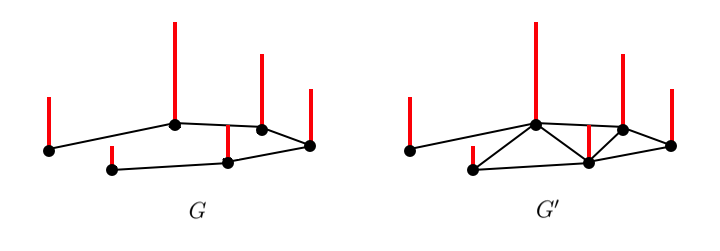
\includegraphics[width=0.8\textwidth]{figs/chapter1/graph.png}
	\caption{\label{fig:graph}Different graph topologies can drastically change the measure of smoothness of a signal $\mathbf f$, here represented as red vertical bars on the vertices.}
\end{figure}

\paragraph{Convolution and filtering on graphs}
 As the plane $\mathbb R^2$ is symmetric with respect to any translation, and the sphere $\mathbb S^2$ is symmetric with respect to any rotation, the respective definitions of convolution are equivariant respectively to these two symmetry groups. Since there are no such global symmetries in a general graph $G$, definitions (\ref{eq:plane convolution}), (\ref{eq:convolution}) can not be extended naturally on graphs. However, both on $\mathbb R^2$ and on $\mathbb S^2$, the convolution of a signal $f$ with a kernel $k$ can be performed in the spectral domain by multiplying the transformed signal $\hat f$ times the transformed kernel $\hat k$: 
\begin{equation}\label{eq:convolution normal}
f*k = \mathcal F^{-1}(\hat f \cdot \hat k)
\end{equation}
In a similar way we can define a notion of convolution also in the graph spectral domain. We use the following definition \cite{Vandergheynst} of the convolution of a signal $\mathbf f$ times a kernel $\mathbf K$:
\begin{equation}\label{eq:graph convolution}
	\Omega_\mathbf K\mathbf f = \mathcal{F}^{-1}_G(\mathbf K \hat {\mathbf f})= \mathbf V\mathbf K  \mathbf V^\intercal {\mathbf f}
\end{equation}
where $\mathbf K$ is a \textit{diagonal} \textit{matrix} $K_{ii} = k_i$. Graphs convolutions are different from the ones we are used to define in Euclidean domains, since the graph kernels $\mathbf K$ are diagonal matrices that can not be thought as the Fourier transform of a corresponding kernel defined in the spatial (vertex) domain. The diagonal elements $k_{i}$ can be thought as functions of the corresponding eigenvalues 
$$
k_{i}= k(\lambda_i)
$$
thus providing an intuitive frequency interpretation of the kernel $\mathbf K$. In this way the convolution can be seen as a \textit{filtering} operation: for example, a kernel $k(\lambda_i) = \exp (-\lambda_i)$ will be the kernel of a low-pass filter since it will cut the high frequencies.

\subsection{The Equivariance error for graph convolutions}
Take a sampling scheme $V=\{v_i\in\mathbb S^2, i=0, ..., n\}$ of the sphere, a weighted undirected graph $G(V, E, \mathbf W)$, a signal $f: \mathbb S^2\to\mathbb R$ and its sampled representation $\mathbf f:\ f_i=f(v_i)$. Suppose that there exists a sampling operator $T_V: L^2(\mathbb S^2) \supset F\to \mathbb R^n,\  T_V(f) = \mathbf f$ defined on a suitable subspace $F$ of $L^2(\mathbb S^2)$ such that it is invertible, i.e., we can unambiguously reconstruct the function $f\in F$ from its sampled values $\mathbf f$. The existence of such subspace depends on the sampling scheme $V$, and its characterization is a common problem in signal processing \cite{Driscoll:1994:CFT:184069.184073}. Recall the definition (\ref{eq:rotation operator}) of the rotation operator $\Lambda(g), g\in SO(3)$. 

We now want to understand how to set the edges and the weights of $G$ such that
\begin{equation}\label{eq:equivariance}
T \Lambda(g) T^{-1} \Omega_k T f = \Omega_k T \Lambda(g) f
\end{equation}
i.e., the graph convolution $\Omega_k$ and any rotation $\Lambda(g)$ commute.

Verifying equation (\ref{eq:equivariance}) is really hard in practice, due to the fact that for almost all samplings schemes $V$ it is not known if there exists a space $F$ in which $T$ is invertible. A special case is the \textit{equiangular sampling} scheme described in section \ref{sec:Chapter3: Heat Kernel Graph Laplacian on the Equiangular Sampling} where the sampling theorem \ref{theo:equiangular sampling theorem} holds \cite{Driscoll:1994:CFT:184069.184073}. With all the other sampling schemes, there are no sampling theorems available, but there are implementations of discrete SHT to reconstruct a sampled signal $\mathbf f$, thus providing a way to approximate $T^{-1}$. Thanks to this we are able, for a given sampling, a given function $f$, a given rotation $g$, and a given kernel $k$, to compute the \textit{normalized equivariance error} 
\begin{equation}\label{eq:equivariance error}
E_{G}(f, g) = \left(\frac{ \norm {T \Lambda(g) T^{-1} \Omega_k Tf - \Omega_k T \Lambda(g) f}_{L^2(\mathbb R^2)}}{\norm {Tf}_{L^2(\mathbb R^2)}}\right)^2
\end{equation}
where $T^{-1}$ is substituted with a discrete SHT in case $T$ is not invertible.
A measure of how equivariant a graph is with respect to rotations will then be given by the \textit{mean equivariance error}
\begin{equation}\label{eq:mean equivariance error}
\overline E_G = \mathbb E_{f, g}\ 	E_G(f, g) 
\end{equation}
In practice the expected value is obtained by averaging over a finite number of random functions and random rotations. The mean equivariance error $\overline E_G$ gives us an indication of how close the graph $G$ is from being equivariant to rotations. Now we state an intuitive concept that explains how to construct rotation invariant graphs, i.e. graphs such that $\overline{E_G}$ is small.
\begin{snugshade*}
	The mean equivariance error $\overline{E_G}$ will be small if the scalar product $\mathbf f^\intercal \mathbf v_{i(\ell, m)}$ well approximates $\hat {f}(\ell,m)$ i.e., the $L^2$ scalar product of the continuous signal \\
	$\hat {f}(\ell,m)= \int_{\eta \in \mathbb S^2}f(\eta)Y_\ell^m(\eta)d\mu(\eta)$.
	
	\textit{If $V$ is an equal area sampling scheme}, i.e. the area around each pixel $v_i$ is the same, $\overline{E_G}$ will be small if the graph Laplacian $\mathbf L$ is such that its eigenvectors $\mathbf v_i$ well approximate the eigenfunctions of the Laplace-Beltrami operator $\Delta_{\mathbb S^2}$ evaluated in the points of the sampling scheme, i.e., 
	$$
	\mathbf v_{i(\ell, m)} \approxeq Y_\ell^m(x_i)
	$$
\end{snugshade*}

In this way we framed the problem of constructing a rotation invariant graph with the more general problem of coming up with a matrix $\mathbf L$ with some specific spectral properties. Graphs are only one of many ways of coming up with such matrix $\mathbf L$, and many other methods have been already studied in the literature. In the next Chapter we present a brief overview of some of these methods providing the general context in which graph filtering can be framed.


\pagebreak


\section{Discrete Laplacians}\label{sec:Chapter3: other discrete laplacians}
In this Chapter we describe different methods to approximate the Laplace-Beltrami operator on manifolds, with particular attention to what we will call the Heat Kernel Graph Laplacian. We need now to introduce some basic concepts of Differential Geometry, especially the definition of mean curvature of a manifold and its link with the Laplace-Beltrami operator.
\subsection{Notions of Differential Geometry}

 For this short introduction to basic concepts of Differential Geometry, set the manifold $\mathcal M$ to be a differentiable, two dimensional surface embedded in $\mathbb R^3$. 
 \begin{figure}[h]
 	\centering
 	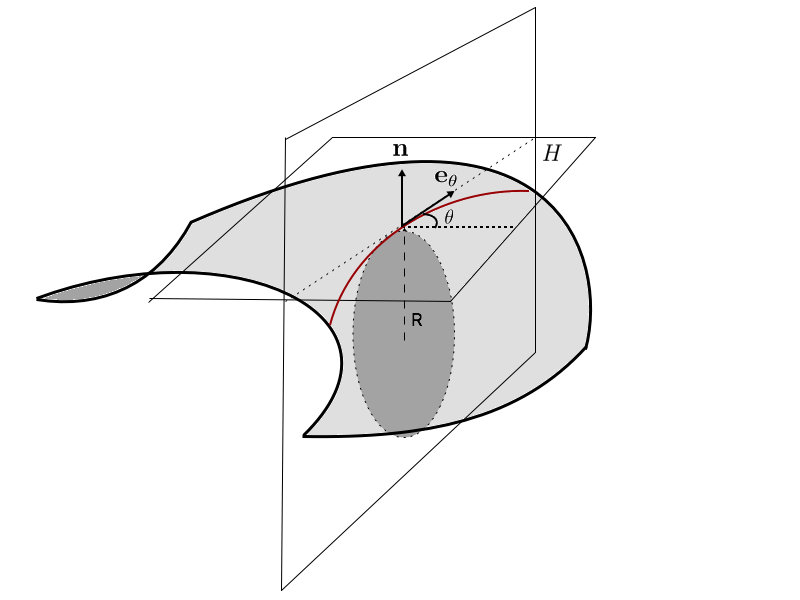
\includegraphics[width=0.7\textwidth]{figs/Chapter3/curvature.png}
 	\caption{\label{fig:curvature}Curvature normal of a manifold}
 \end{figure} 
The \textit{curvature} of a curve on a plane is defined as the inverse of the radius $R$ of the tangent circle. For each point on the manifold $\mathcal M$, define its tangent plane $H$, orthogonal to the normal vector $\mathbf n$. For every unit vector $\mathbf e_\theta$ lying on the tangent plane $H$, where $\theta$ is an angle that measures the direction on the tangent plane of $\mathbf e_\theta$, the \textit{normal curvature} $\kappa(\theta)$ is defined as the curvature of the curve that is the intersection of the manifold $\mathcal M$ and the plane containing both $\mathbf n$ and $\mathbf e_\theta$. The \textit{mean curvature} $\overline \kappa $ is defined as the average on $\theta$ of the normal curvatures:
 
 \begin{equation}\label{eq:mean curvature}
 	\overline \kappa=\frac{1}{2 \pi} \int_{0}^{2 \pi} \kappa(\theta) d \theta
 \end{equation}

It can be proved that the Laplace-Beltrami operator applied on the identity function $\mathbf x \rightarrow \mathbf x, \ \forall \mathbf x\in \mathcal M$ is directly linked to the \textit{mean curvature normal} $\overline{\kappa}\mathbf n$ by the following formula:
\begin{equation}\label{eq:laplacian and curvature}
	\triangle_\mathcal M \mathbf x  = -2\overline{\kappa}\mathbf n
\end{equation}
This equation provides us a way to approximate the Laplace-Beltrami operator through the approximation of the mean curvature normal. This fact is exploited by methods presented in the next section.

\subsection{Discrete Laplacians from Differential Geometry}
\begin{figure}[h]
	\begin{center}
		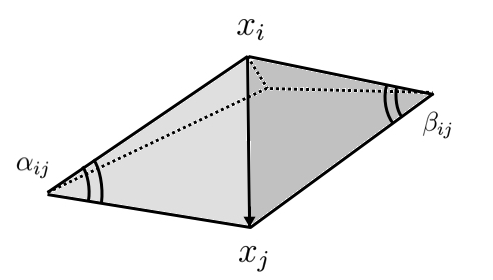
\includegraphics[width=0.45\textwidth]{figs/Chapter3/MyDesbrun.png}
		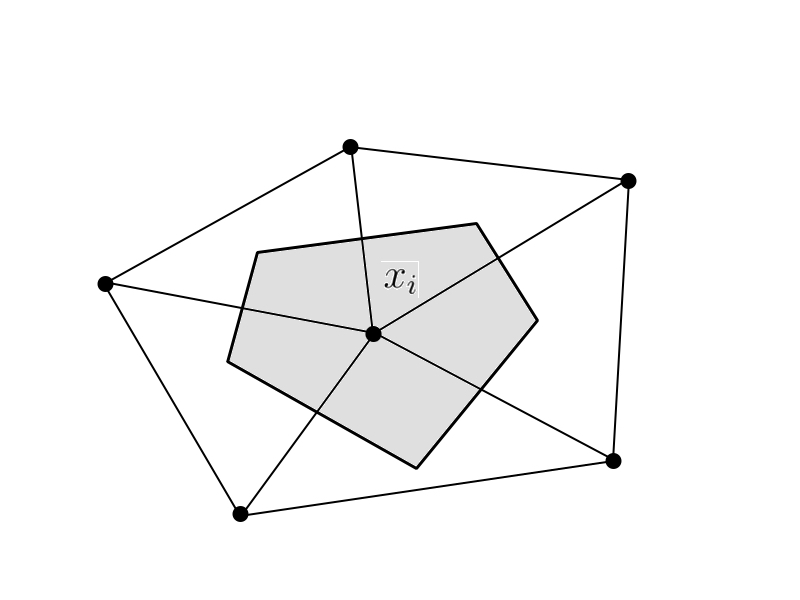
\includegraphics[width=0.45\textwidth]{figs/Chapter3/Voronoi}
	\end{center}
	\caption{\label{fig:Desbrun}One term of curvature normal formula and one Voronoi cell constructed around the node $x_i$}
\end{figure} 
Desbrun et al. \cite{Desbrun1999} construct a triangulation $\mathcal T_h$ with the vertices in the sampling $x_0, x_1, ..., x_{n-1}$ approximating the manifold $\mathcal M$, and then use the following discrete expression for the \textit{discrete normal curvature} $\overline{\kappa_h} \mathbf{n}$ of the manifold $\mathcal M$:
\begin{equation}\label{eq:curvature normal}
	-\overline{\kappa_h} =\frac{1}{4 A_i} \sum_{j \in N_{1}(i)}\left(\cot \alpha_{ij}+\cot \beta_{ij}\right)\left(x_{j}-x_{i}\right)
\end{equation}
where $A_i$ is the area of all the triangles of the mesh sharing the node $x_i$; $N_1(i)$ is the first ring of neighbors of the i-th node; $\alpha_{i j},\ \beta_{i j}$ are the angles of the triangles of the mesh that lie on the opposite side to the edge $(i,j)$ with respect to the node $x_i$ (Figure \ref{fig:Desbrun}). Observe that for a flat surface the discrete curvature is equal to zero $\overline{\kappa_h}=0$. This is a geometric approach that relies on the intrinsic properties of the triangulation $\mathcal T_h$ and is based on the geometric meaning of the curvature normal $\overline{\kappa}$. Using equations (\ref{eq:curvature normal}) and (ref{eq:laplacian and curvature}) it can be shown \cite{REUTER2009381} that this approach leads to a \textit{discrete Laplacian} with masses $d_i=A_i$ where $A_i$ is the area of all the triangles of the mesh with a node in $x_i$, and weights
$$
w_{i j}=\frac{\cot \left(\alpha_{i j}\right)+\cot \left(\beta_{i j}\right)}{2}
$$

Meyer et al. \cite{Meyer02discretedifferential-geometry} modify the masses of Desbrun et al. and set the masses $d_i$ to be equal to $a_{V}(i)$, where \(a_{V}(i)\) is the area of the polygon obtained by joining the circumcenters of the triangles surrounding node $i$ (i.e. the Voronoi cell, figure \ref{fig:Desbrun}).

\subsection{Linear Finite Element Method Laplacian}
The eigenvalue problem (\ref{eq:continous eigenvalue problem}) can be rewritten in the equivalent weak form
\begin{equation}\label{eq:weak}
	\langle \nabla f, \nabla v\rangle_{L^2(\mathbb S^2)} = \lambda \langle  f, v\rangle_{L^2(\mathbb S^2)} \quad \forall v \in L^2(\mathbb S^2)
\end{equation}
The Finite Element Method (FEM) is a numerical algorithm that allows to calculate a discrete approximation of the solution $f$ through a functional discretization of the weak eigenvalue problem (\ref{eq:weak}). We will discuss this method deeper in section \ref{sec:Chapter3: Using the Finite Element Method to approximate the Laplace-Beltrami operator on a manifold}. By projecting equation (\ref{eq:weak}) on a finite dimensional functional subspace of $L^2(\mathbb S^2)$ spanned by $n$ basis functions $\phi_i$, by writing $n$ times the equation (\ref{eq:weak eigenvalue problem}), setting each time the \textit{test} function $v$ equal to the $i$th basis function $\phi_i$ we obtain the generalized algebraic eigenvalue problem
$$
\begin{aligned}
&\text{Find }(f,\lambda)\text{ such that }A\mathbf f = \lambda B \mathbf f\\
&\begin{cases}
(A)_{ij} &= \int_{\mathbb S^2}\nabla \phi_i(\mathbf{x})\cdot \nabla \phi_j(\mathbf{x})d\mathbf{x}\\
(B)_{ij} &= \int_{\mathbb S^2} \phi_i(\mathbf{x}) \phi_j(\mathbf{x})d\mathbf{x}\\
(\mathbf f)_i &= f_i:\quad f(\mathbf x) = f_0\phi_0(\mathbf x)+ ... + f_{n-1}\phi_{n-1}(\mathbf x) 
\end{cases}
\end{aligned}
$$
that can be solved through usual algebraic solvers.

\subsection{Graph Laplacian for manifolds}\label{sec:Chapter1:theoretical foundations}
In their work, Convergence of Laplacian Eigenmaps \cite{NIPS2006_2989}, Belkin et al. prove convergence of eigenvectors of the \textit{Heat Kernel Graph Laplacian} $\mathbf L_n^t$ (HKGL) of a data point cloud to the eigenfunctions of the Laplace Beltrami operator $\Delta_\mathcal M$ on the manifold $\mathcal M$, when the data is sampled from a uniform distribution on $\mathcal M$.
For this result to hold, they suppose the manifold $\mathcal M$ to be compact, infinitely differentiable and without boundary. We just point out that being $\mathcal M$ compact, $\Delta_\mathcal M$ has a discrete spectrum. The graph they use to approximate the manifold is constructed as follows: given a sampling $ \mathcal P = \{x_i\in\mathcal M\}_{i=0}^{n-1}$ on a $k$-dimensional manifold $\mathcal M\subset \mathbb R^N$ they construct the full graph defined by the weights 
$$
w_{ij}=\exp\left({-\frac{||x_i-x_j||^2}{4t}}\right)
$$
where $\norm\cdot$ is the Euclidean norm in the ambient space $\mathbb R^N$ and whose Laplacian matrix 
$$
\mathbf L_n^t = \mathbf D-W
$$ we call \textit{Heat Kernel Graph Laplacian}.

Observe that given a function $f: \mathcal P \rightarrow \mathbb R$ defined on the sampling $ \mathcal P$ and defined the vector $\mathbf f\in\mathbb R^n$ such that $\mathbf f_i = f(x_i)$, the Heat Kernel Graph Laplacian matrix acts on $\mathbf f$ in the following way:
\begin{equation}\label{eq:HKGL}
(\mathbf L_n^t \mathbf f)_i:=  \sum_{j=0}^{n-1} e^{-\frac{||x_i-x_j||^2}{4t}}\left(f(x_i)-f(x_j)\right)
\end{equation}
This graph construction is motivated by the fact that the HKGL is nothing else than the natural discretization of the continuous \textit{functional approximation to the Laplace-Beltrami operator} $L^t:  L^{2}(\mathcal{M}) \rightarrow L^{2}(\mathcal{M})$ that is proven to converge to $\Delta_\mathcal M$.
\vspace{0.5cm}
\begin{definition}{}(\cite[Belkin et al.]{Belkin:2005:TTF:2138147.2138189}Functional approximation to the Laplace-Beltrami operator)\\ \label{eq: my L^t} Let $\mu$ be the uniform probability measure on the manifold $\mathcal M$, where $\text{vol}(\mathcal M)$ is the volume of $\mathcal M$. We define the functional approximation to the Laplace-Beltrami operator to be the operator $L^t: L^{2}(\mathcal{M}) \rightarrow L^{2}(\mathcal{M})$ such that
	\label{def:Functional approximation to the Laplace-Beltrami operator}
	$$ L^tf(y) = \int_{\mathcal M}e^{-\frac{||y-x||^2}{4t}}\left(f(y)-f(x)\right)d\mu(x)$$
\end{definition}
We end this Chapter by stating the theorem of spectral convergence of the HKGL to the Laplace-Beltrami operator $\Delta_\mathcal M$, that makes it a really good candidate to construct rotation invariant graphs.
\vspace{0.5cm}
\begin{snugshade*}
	\begin{theorem}(Belkin et al., \cite{NIPS2006_2989})\label{theo:spectral convergence}
		Let \(\lambda_{n, i}^{t}\) be the $i$th eigenvalue of 
		$$
		\frac{(4\pi t)^{-(k+2)/2}}{n}\mathbf L^t_n
		$$
		and \(\mathbf v_{n, i}^{t}\) be the corresponding eigenvector. Let \(\lambda_{i}\) and \(v_{i}\) be the corresponding eigenvalue and eigenfunction of \(\Delta\) respectively. Then there exists a sequence \(t_{n} \rightarrow 0,\) such that
		\begin{equation}
		\begin{array}{c}{\lim _{n \rightarrow \infty} \lambda_{n, i}^{t_{n}}=\lambda_{i}} \\ 
		{\lim _{n \rightarrow \infty}\left\|\mathbf v_{n, i}^{t_{n}}-v_{i}(\mathbf x)\right\|_{2}=0}\end{array}
		\end{equation}
		where the limits are in probability.
	\end{theorem}
\end{snugshade*}





\pagebreak


%*******************************************************************************
%*********************************** First Chapter *****************************
%*******************************************************************************
%!TEX root = 0.main.tex

\section{Improving Deep Sphere}
\subsection{Adapting Belkin's setting to HEALPix sampling}
\subsubsection*{Pointwise convergence of the Graph Laplacian in the HEALPix case}
\subsubsection*{About the kernel width $t$}
Here we discuss how a big $t$ better captures the low frequencies, a smaller one captures the high frequencies up to the nearest neighbors.
\subsubsection*{Reducing the number of neighbors}
Here we present our final result obtained by thresholding the weights
\subsection{Experimental validation}
Here we report Frederick's results with the two different constructions


\pagebreak


%*******************************************************************************
%*********************************** Second Chapter ***************************
%*******************************************************************************
%!TEX root = 0.main.tex

\section{Other samplings and other Discrete Laplacians}

[What we want from the Laplacian matrix]\\
In a Graph Spherical CNN we use the fact that when the sampling of the sphere is regular enough, the graph $W_{i j} = \exp {-\frac{\norm{x_i-x_j}^2}{4t}}$ is such that the corresponding graph Laplacian $\mathbf L_n^t=D-W$ has a spectrum that is close enough to the spectrum of $\triangle$ so that we can approximate a spherical convolution of a signal with a kernel with a multiplication of a polynomial of the discrete Laplacian $\sum_k \theta_k (\mathbf L_n^t)^k$ times the vector of the sampled signal $\mathbf f_i = f(x_i)$. 

[Stating the problem we want to solve]\\
In Chapter 2 we showed a way to construct $\mathbf L_n^t$ that well approximates $\triangle$ in the case of a much regular sampling of the sphere, HEALPix. In this Chapter we focus to others samplings less uniform than HEALPix. The sampling that we will use for our study, very used in applications, is the so called equiangular sampling. We will observe that in this case the Heat Kernel Graph Laplacian matrix is not able to correctly approximate the continuous Laplace-Beltrami operator, due to the fact that the equiangular sampling samples some specific areas of the sphere more than others. The goal of this chapter is to find a way of building a discrete approximation $\mathbf L$ of the Laplace-Beltrami operator more robust to non uniform sampling than the Heat Kernel Graph Laplacian matrix $\mathbf L_n^t$ used so far.

[Say what we did to solve it]\\
This chapter is organized as follows: In Section \ref{sec:Chapter3: Heat Kernel Graph Laplacian on the Equiangular Sampling} we introduce the equiangular sampling and the results that we obtained with the Heat Kernel Graph Laplacian matrix. In Section \ref{sec:Chapter3: other discrete laplacians} we present a short overview of different ways of building an discrete approximation of the Laplace-Beltrami operator; in Section \ref{sec:Chapter3: Using the Finite Element Method to approximate the Laplace-Beltrami operator on a manifold} we deepen how to use the Finite Element Method (FEM) to construct a discrete approximation of $\triangle$ and how this way of constructing $\mathbf L$  is actually capable of taking into account the non uniformity of the sampling and correct it. in Section \ref{sec:Chapter3: Results} we present and discuss the results obtained.
\subsection{Heat Kernel Graph Laplacian on the Equiangular Sampling}
\label{sec:Chapter3: Heat Kernel Graph Laplacian on the Equiangular Sampling}

\subsubsection{The Equiangular Sampling}
[Present the equiangular sampling]\\
Given the usual parametrization $x = x(\theta, \phi)$ of the sphere
$$
\mathbb{S}^{2}=\left\{x=\left(x_{1}, x_{2}, x_{3}\right) \in \mathbb{R}^{3} :\|x\|_{\mathbb{R}^{3}}=\left(x_{1}^{2}+x_{2}^{2}+x_{3}^{2}\right)^{1 / 2}=1\right\}
$$

$$
x_{1}=\cos (\phi) \sin (\theta), \quad x_{2}=\sin (\phi) \sin (\theta), \quad x_{3}=\cos (\theta)
$$
Let $m\in\mathbb N$, the uniform sampling of bandwidth $b=2^m$ is given by 
$
x_{j k}^{(b)}=x\left(\theta_{j}^{(b)}, \phi_{k}^{(b)}\right)
$
where
$$
\theta_{j}^{(b)} :=\pi \frac{j}{2 b}, \quad \phi_{k}^{(b)} :=2 \pi \frac{k}{2 b}
$$
\begin{figure}[h!]
	\centering
	\label{fig:equiangular sampling}
	\caption{Equiangular sampling with bandwidth $n=16$}
	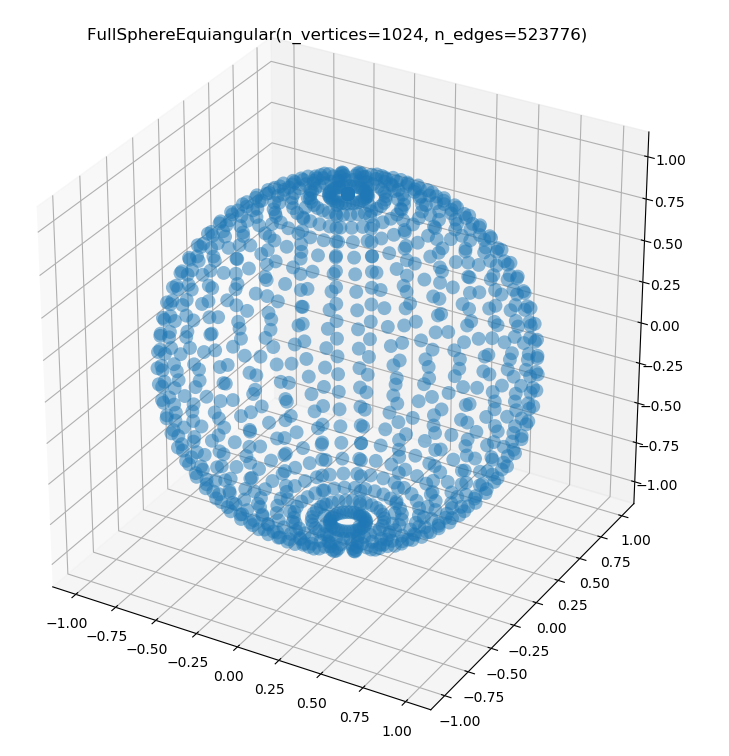
\includegraphics[width=0.5\textwidth]{../codes/02.HeatKernelGraphLaplacian/equiangular/equiangular.png}
\end{figure}
One has $n=4b^2$ points on the sphere, where $x_{0 k}^{(b)}$ corresponds to the north pole for every $k$. Notice also that the south pole is never sampled. In figure \ref{fig:equiangular sampling} it can also be appreciated how the area close to the poles is much more sampled that the equator. One reason for which this sampling is very useful is the following result from \cite{Driscoll:1994:CFT:184069.184073}, that states that any band limited function can be exactly recovered from its sampled values $f\left(x_{j k}^{(b)}\right)$:
\vspace{0.5cm}
\begin{prop}\label{prop:equiangular sampling theorem}
	Let \(l_{0} \in \mathbb{N}\) and \(m_{0} \in \mathbb{Z},\left|m_{0}\right| \leq l_{0} .\) If \(f=\sum_{l=0}^{b-1} \sum_{m=-l}^{l} \widehat{f}(l, m) Y_{l}^{m}\)
	then
	
	$$
	\begin{aligned} \widehat{f}\left(l_{0}, m_{0}\right)=& \frac{1}{4 b^{2}} \sum_{j=0}^{2 b-1} \sum_{k=0}^{2 b-1} f\left(x_{j k}^{(b)}\right) \overline{Y_{l_{0}}^{m_{0}}\left(x_{j k}^{(b)}\right)} \sin \left(\theta_{j}^{(b)}\right) \times \\ & \times \frac{4}{\pi} \sum_{l=0}^{b-1} \frac{1}{2 l+1} \sin \left((2 l+1) \theta_{j}^{(b)}\right) \end{aligned}
	$$
\end{prop}
\vspace{0.5cm}

\subsubsection{Heat Kernel Graph Laplacian}
Thanks to Proposition \ref{prop:equiangular sampling theorem}, assuming we can compute the Fourier transform of the eigenvectors of the Heat Kernel Graph Laplacian matrix and see how much they are aligned with the eigenspaces of the true Laplace-Beltrami operator. Here the results:


\begin{table}[h!]
	\centering
	\label{table:equiangular kernel width}
	\caption{Kernel width $t$ used to construct the Heat Kernel Graph Laplacian matrix fr each bandwidth $b$}
	\begin{tabular}{ c|c } 
	
$b$ & $t$ \\ 
	\hline
4 & 0.5 \\ 
8 & 0.3 \\ 
16 & 0.1 \\ 
	
	\end{tabular}
\end{table}

\begin{figure}[h!]
	\centering
	\label{fig:equiangular sampling alignment}
	\caption{Alignment of eigenspaces of the Heat Kernel Graph Laplacian matrix with the true Laplace-Beltrami eigenspaces on the equiangular sampling with $b=16$ and kernel width $t=0.1$}
	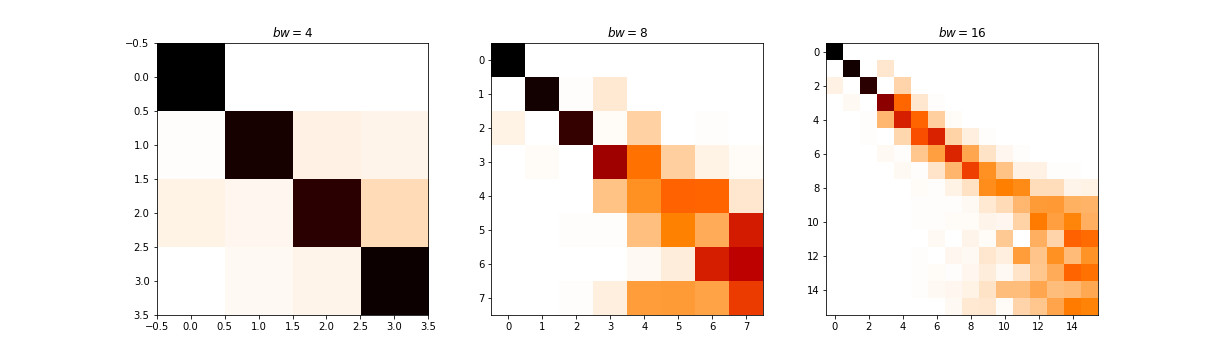
\includegraphics[width=0.9\textwidth]{../codes/02.HeatKernelGraphLaplacian/equiangular/equi_full.png}
\end{figure}
\begin{figure}[h!]
	\centering
	\label{fig:equiangular sampling alignment diagonal}
	\caption{Alignment of eigenspaces of the Heat Kernel Graph Laplacian matrix with the true Laplace-Beltrami eigenspaces on the equiangular sampling}
	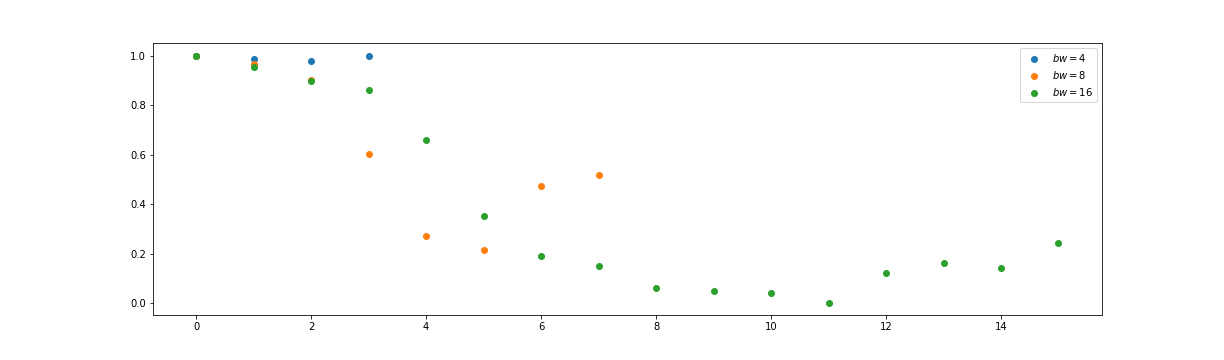
\includegraphics[width=0.9\textwidth]{../codes/02.HeatKernelGraphLaplacian/equiangular/equi_full_diagonal.png}
\end{figure}
\begin{figure}[h!]
	\centering
	\label{fig:equiangular sampling alignment eigenvalues}
	\caption{Eigenvalues of the Heat Kernel Graph Laplacian matrix on the equiangular sampling with $b=16$ and kernel width $t=0.1$}
	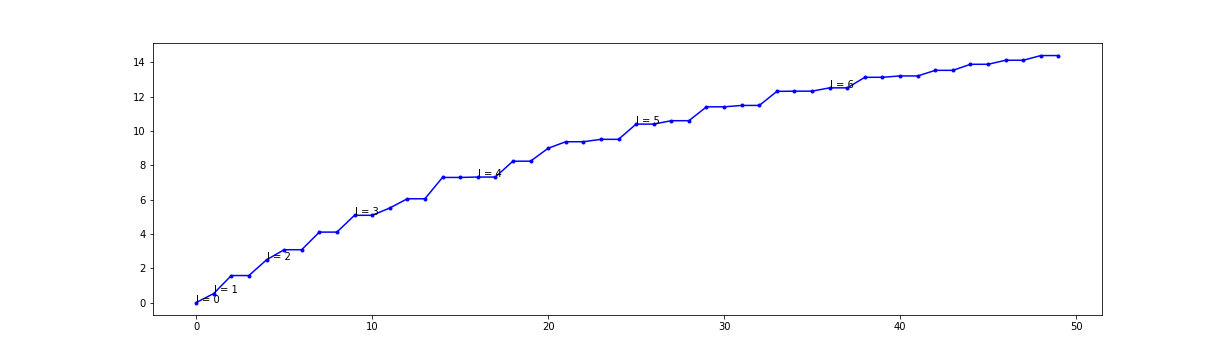
\includegraphics[width=0.9\textwidth]{../codes/02.HeatKernelGraphLaplacian/equiangular/equi_full_eigenvalues_16.png}
\end{figure}

It can be appreciated how poor these results are compared to the ones obtained with the HEALPix sampling. \\

[ Explain why they are so bad: Perspective of the quadrature formula]\\
A way to understand what's going on is the following: remembering the proof of theorem \ref{theo:pointwise convergence in the healpix case} and using again the notation $\phi^{t}(x ; y)=e^{-\frac{||x-y||^2}{4t}}\left(f(y)-f(x)\right)$, the key thing is to make $L_n^tf(y)=\sum_i \frac{1}{n} \phi^{t}(x_i ; y)$  approximate $L^tf(y)=\int_\mathcal M\phi^{t}(x ; y)d\mu(x)$, in other words we can see the graph weights as \textit{quadrature weights} meant to approximate the continuous integral on the right hand side of equation \ref{eq:quadrature approximation}.
\begin{equation}
\label{eq:quadrature approximation}
	\sum_i \frac{1}{n} \phi^{t}(x_i ; y) \quad \approxeq\quad \int_\mathcal M\phi^{t}(x ; y)d\mu(x)
\end{equation}
The way of building the graph of Belkin et al. works in the case of random sampling because in that way the sampling in the limit of the SLLN will sample the manifold uniformly, and thus there's no need of re-weighting the graph; in case of non uniform sampling, we intuitively need to modify the Heat Kernel weights $W_{i j}=e^{-\frac{\norm{x_i-x_j}^2}{4t}}$ with some coefficients $\alpha_i$ to create a re-weighted graph 
$$
W'_{i j} = \alpha_i W_{i j}
$$

in order for $L_n^tf(y)$ to correctly approximate $L^tf(y)$, where $\alpha_i$ would be smaller in pixels that are in areas closer to the poles and bigger in areas closer to the equator. 

\begin{equation}
\label{eq:quadrature approximation 2}
\sum_i \frac{1}{n} \alpha_i \phi^{t}(x_i ; y) \quad \approxeq\quad \int_\mathcal M  \phi^{t}(x ; y)d\mu(x)
\end{equation}
In the next section we present some different ways of building the matrix $\mathbf L$.

\clearpage
\subsection{Other Discrete Laplacians}\label{sec:Chapter3: other discrete laplacians}
Present all the other ways of approximating the Laplace-Beltrami operator you found: graphs, Laplace de Rham, FEM
\subsubsection{Frossard/Khasanova graph}
\begin{figure}[h]
	\label{fig:Frossard/Khasanova graph}
	\centering
	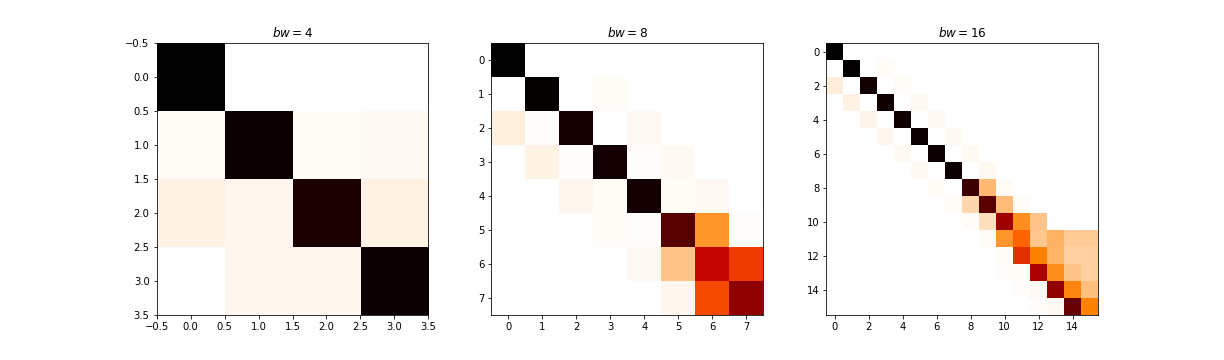
\includegraphics[width=0.9\textwidth]{../codes/02.HeatKernelGraphLaplacian/equiangular/equi_Khasanova_Frossard_full.png}
	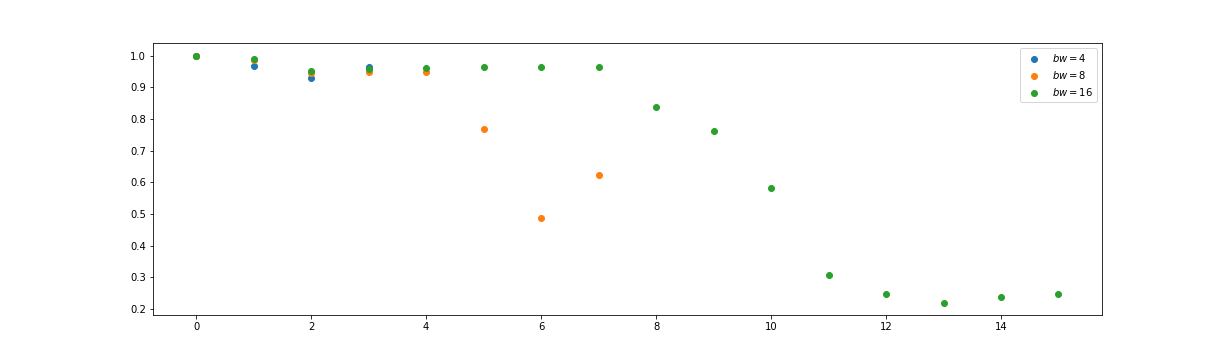
\includegraphics[width=0.9\textwidth]{../codes/02.HeatKernelGraphLaplacian/equiangular/equi_Khasanova_Frossard_full_diagonal.png}
	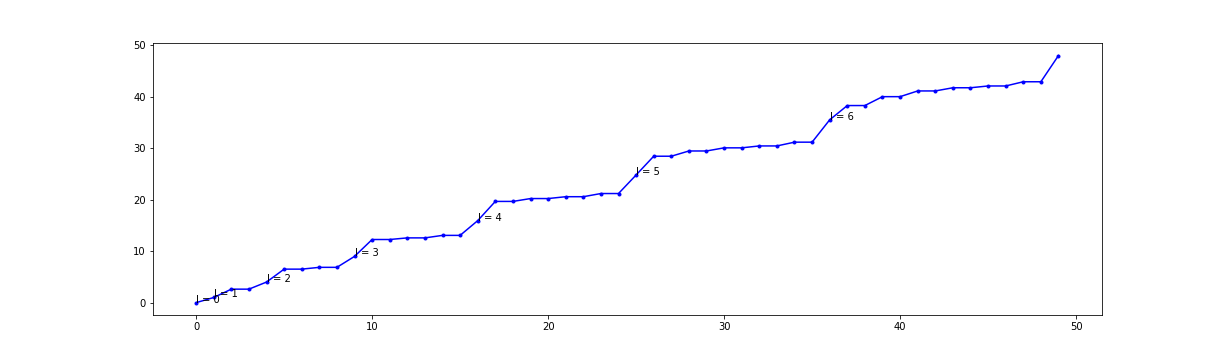
\includegraphics[width=0.9\textwidth]{../codes/02.HeatKernelGraphLaplacian/equiangular/equi_full_Khasanova_Frossard_eigenvalues_16.png}
	\caption{Frossard/Khasanova graph}
\end{figure}
\begin{figure}[h]
	\label{fig:Frossard/Khasanova geodesic graph}
	\centering
	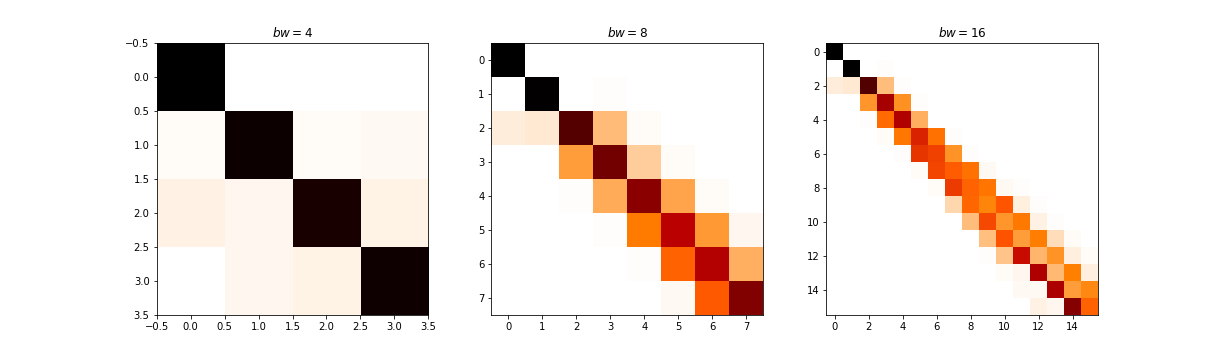
\includegraphics[width=0.9\textwidth]{../codes/02.HeatKernelGraphLaplacian/equiangular/equi_Khasanova_Frossard_full_geodesic.png}
	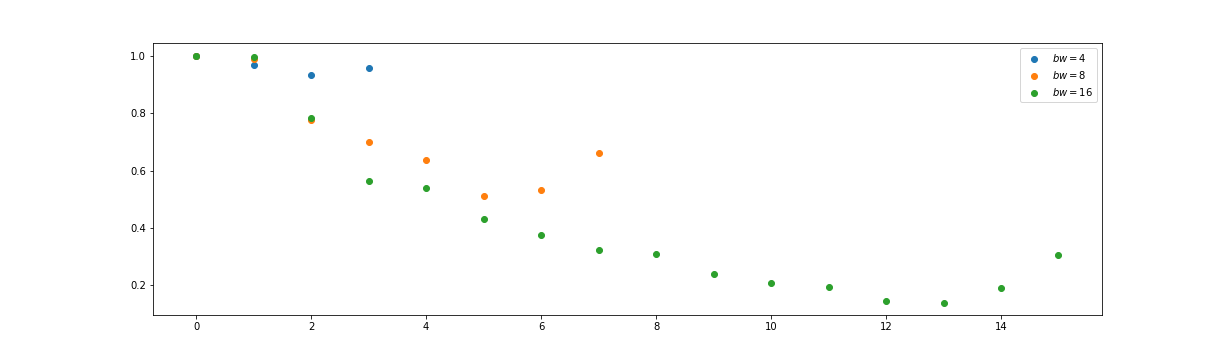
\includegraphics[width=0.9\textwidth]{../codes/02.HeatKernelGraphLaplacian/equiangular/equi_Khasanova_Frossard_full_diagonal_geodesic.png}
	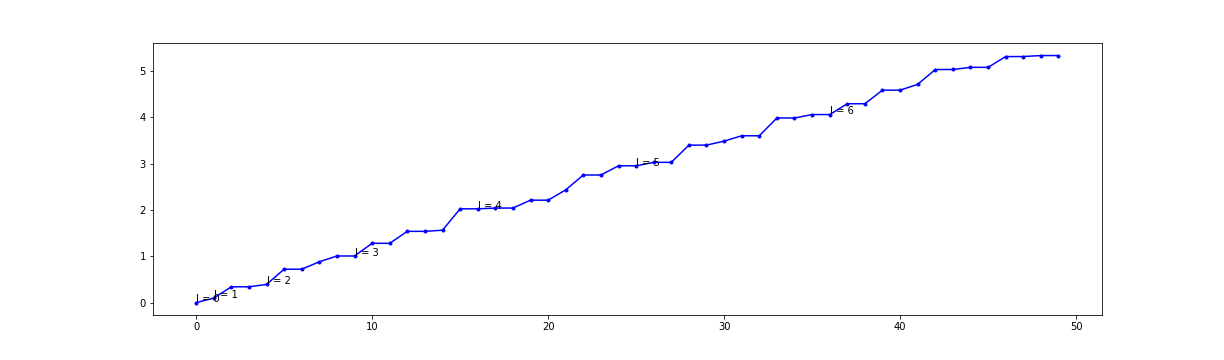
\includegraphics[width=0.9\textwidth]{../codes/02.HeatKernelGraphLaplacian/equiangular/equi_full_Khasanova_Frossard_eigenvalues_16_geodesic.png}
	\caption{Frossard/Khasanova geodesic graph}
\end{figure}
\subsection{Using the Finite Element Method to approximate the Laplace-Beltrami operator on a manifold}\label{sec:Chapter3: Using the Finite Element Method to approximate the Laplace-Beltrami operator on a manifold}
Basic ingredients: works on a mesh, 
\subsubsection{Galerkin Method and Finite Element Method}
General introduction to the FEM: definitions, weak formulation, functional spaces, Galerkin method, linear FEM.
\subsubsection{The eigenvalue problem on a manifold}
Weak formulation of the eigenvalue problem on the sphere, generalized eigenvalue problem, lumping of the mass matrix, discussion on the solvers
\begin{figure}[h]
	\label{fig:Lumping}
	\centering
	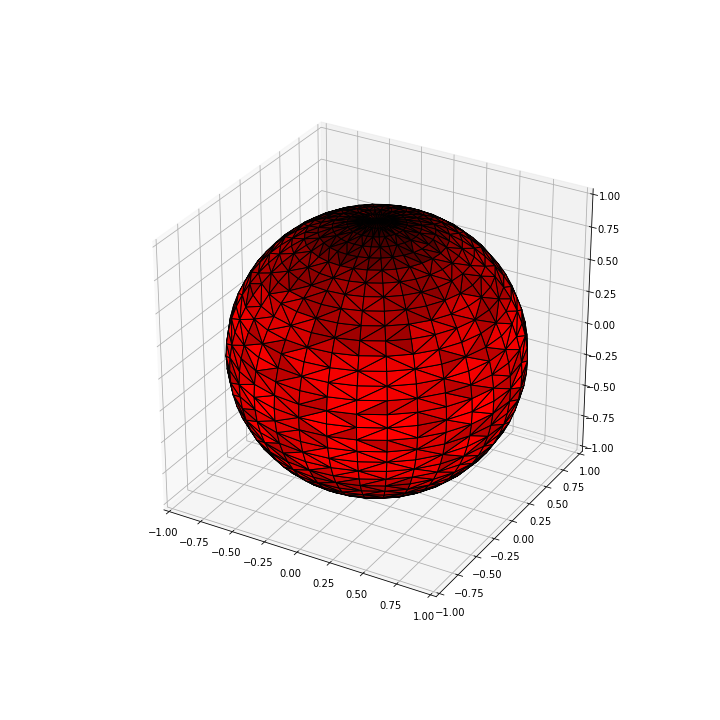
\includegraphics[width=0.9\textwidth]{../codes/03.FEM_laplacian/equiangular/normal/img/mass_matrix_diagonal.png}

	\caption{Diagonal of the lumped mass matrix}
\end{figure}
\subsection{Results}
\label{sec:Chapter3: Results}

\subsubsection{Alignment of eigenspaces and analysis of the spectra}

\paragraph{HEALPix}
\begin{figure}[h]
	\label{fig:HeatKernelGraphLaplacianHealpix}
	\centering
	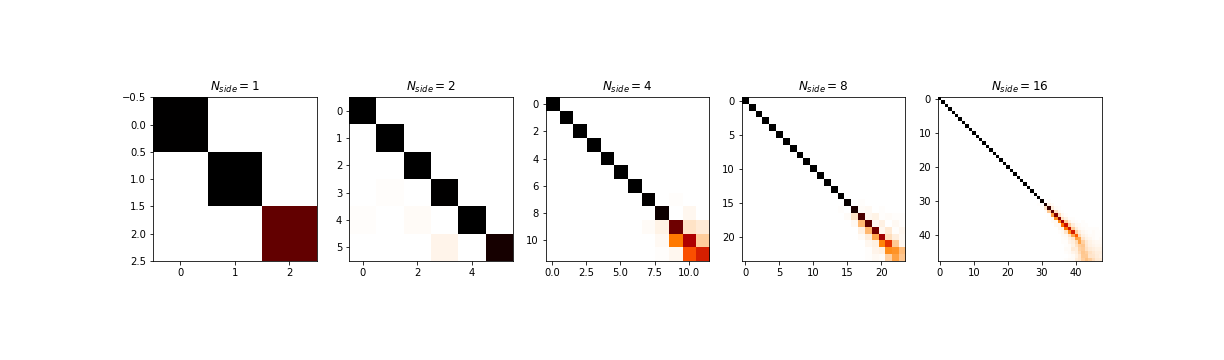
\includegraphics[width=0.9\textwidth]{../codes/02.HeatKernelGraphLaplacian/HEALPix/06_figures/optimal_thresholded.png}
	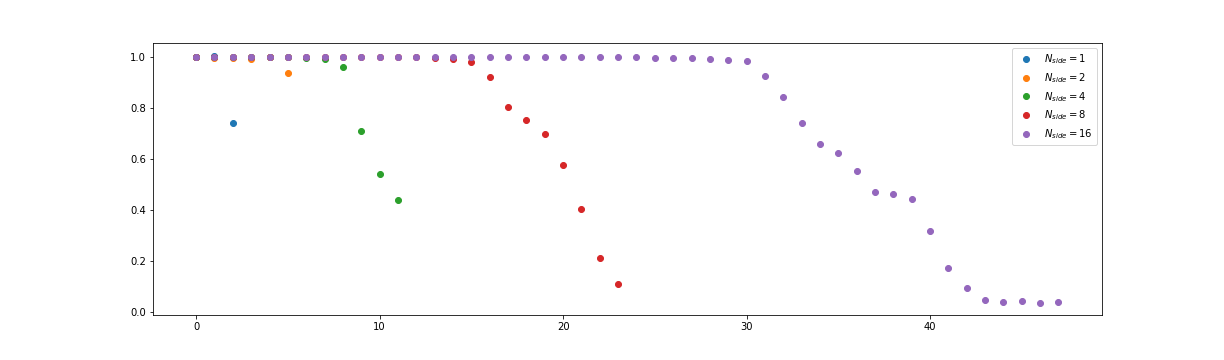
\includegraphics[width=0.9\textwidth]{../codes/02.HeatKernelGraphLaplacian/HEALPix/06_figures/optimal_thresholded_diagonal.png}	
	\caption{Heat Kernel Graph Laplacian on HEALPix}
\end{figure}

\begin{figure}[h]
	\label{fig:FEMHealpix}
	\caption{Linear FEM Laplacian on HEALPix}
	\centering
	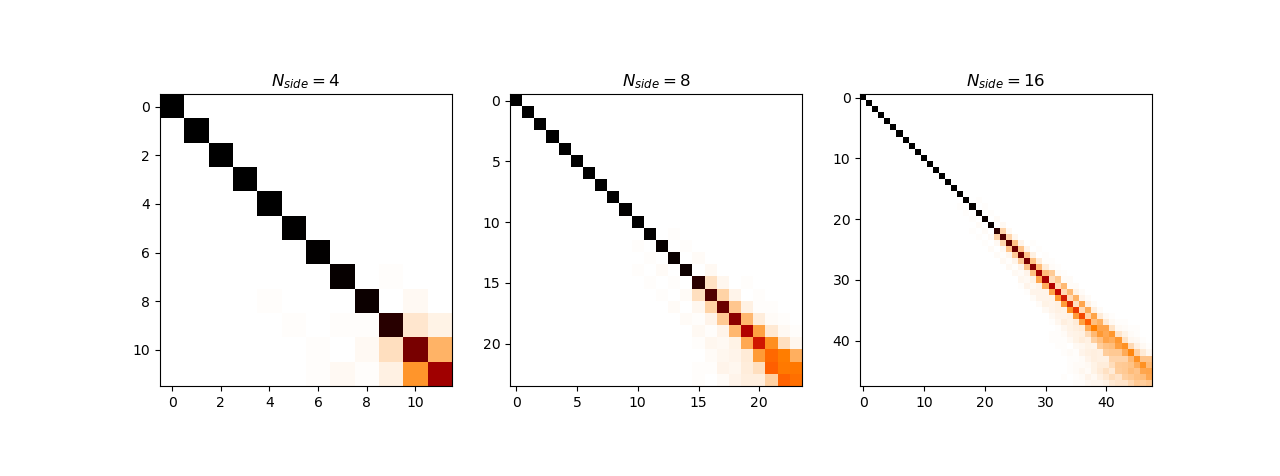
\includegraphics[width=0.8\textwidth]{../codes/03.FEM_laplacian/HEALPix/img/linearFEM.png}
	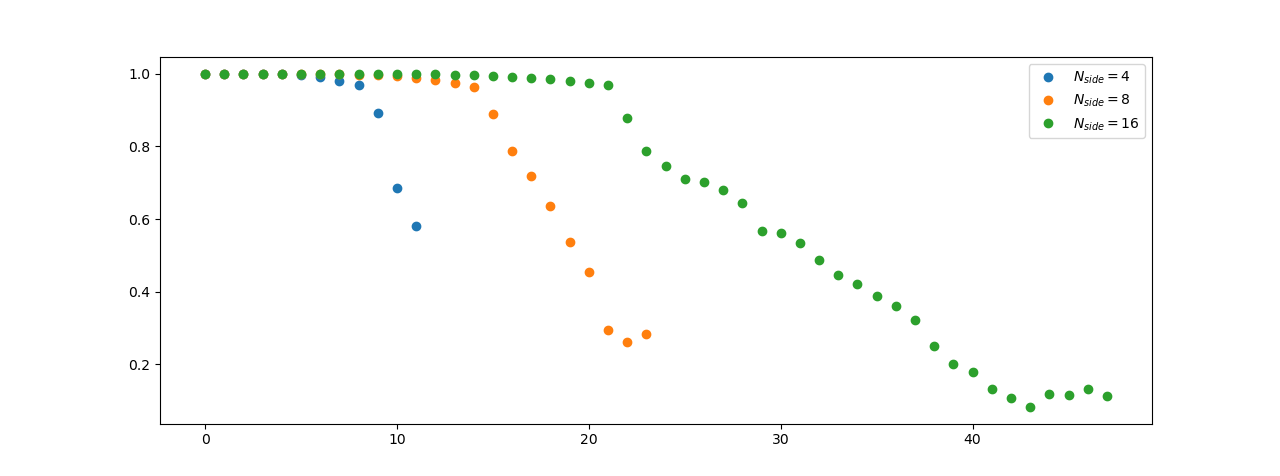
\includegraphics[width=0.8\textwidth]{../codes/03.FEM_laplacian/HEALPix/img/linearFEM_diagonal.png}	
	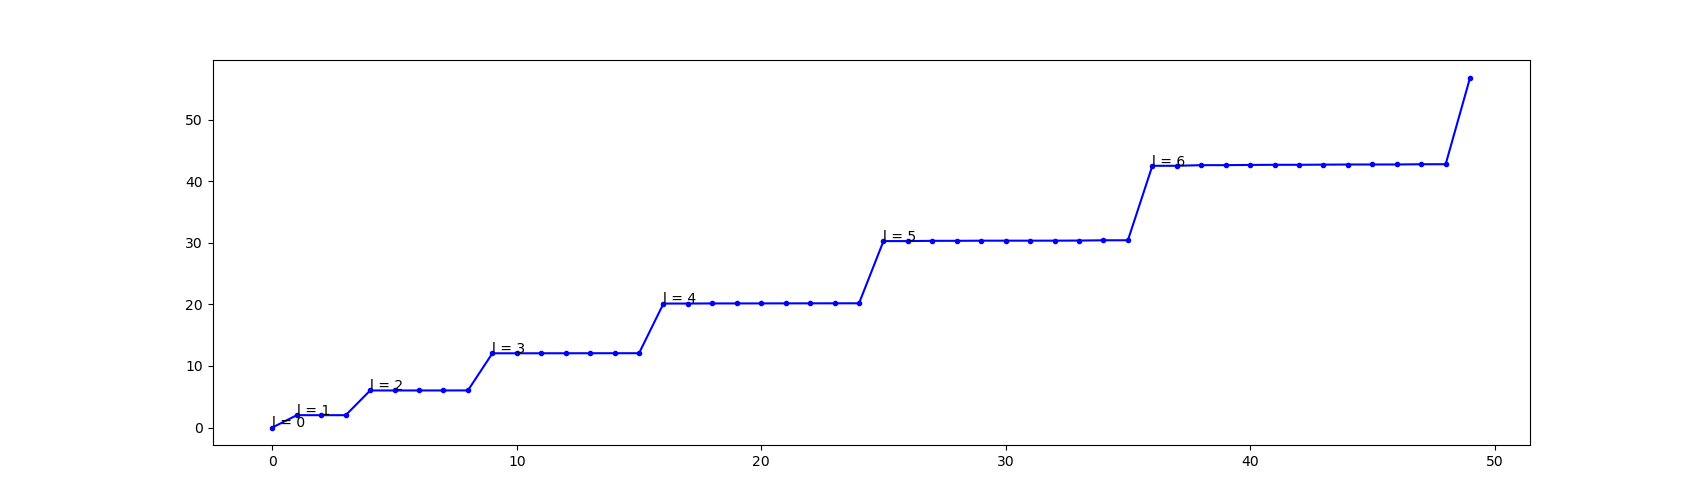
\includegraphics[width=0.8\textwidth]{../codes/03.FEM_laplacian/HEALPix/img/FEM_eigenvalues_16.png}	 
\end{figure}

\paragraph{Equiangular}
\begin{figure}[h]
	\label{fig:HeatKernelGraphLaplacianEquiangular}
	\caption{Heat Kernel Graph Laplacian on equiangular sampling}
	\centering
	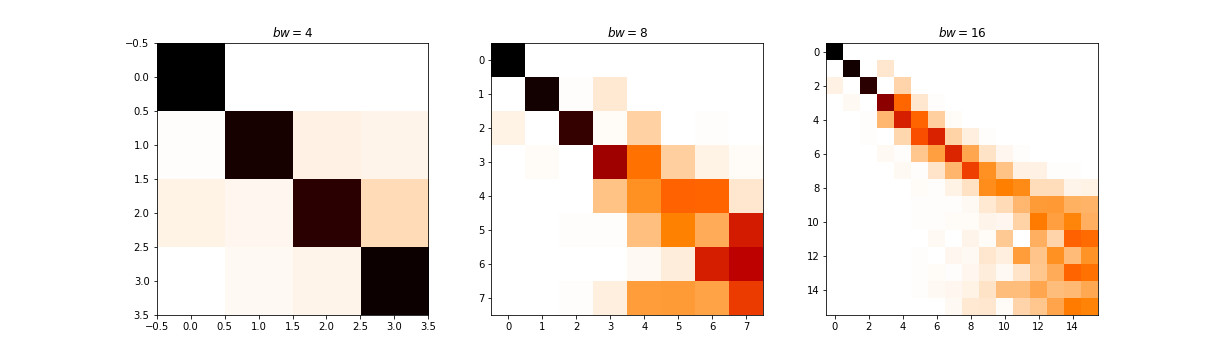
\includegraphics[width=0.9\textwidth]{../codes/02.HeatKernelGraphLaplacian/equiangular/equi_full.png}
	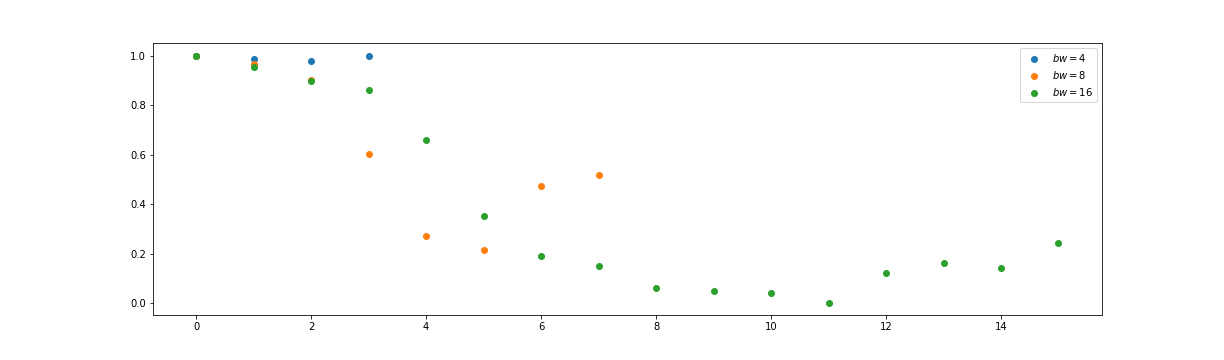
\includegraphics[width=0.9\textwidth]{../codes/02.HeatKernelGraphLaplacian/equiangular/equi_full_diagonal.png}	
	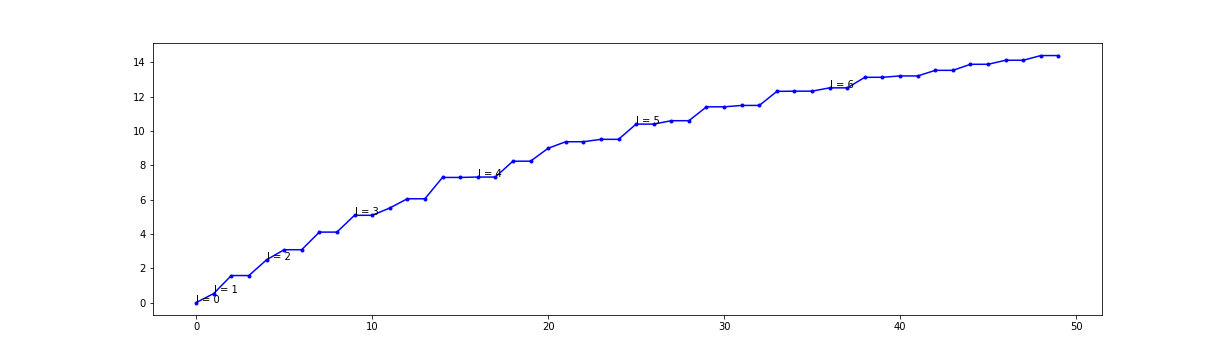
\includegraphics[width=0.9\textwidth]{../codes/02.HeatKernelGraphLaplacian/equiangular/equi_full_eigenvalues_16.png}	
\end{figure}


\begin{figure}[h]
	\label{fig:FEMequiangular}
	\caption{Linear FEM Laplacian on equiangular sampling}
	\centering
	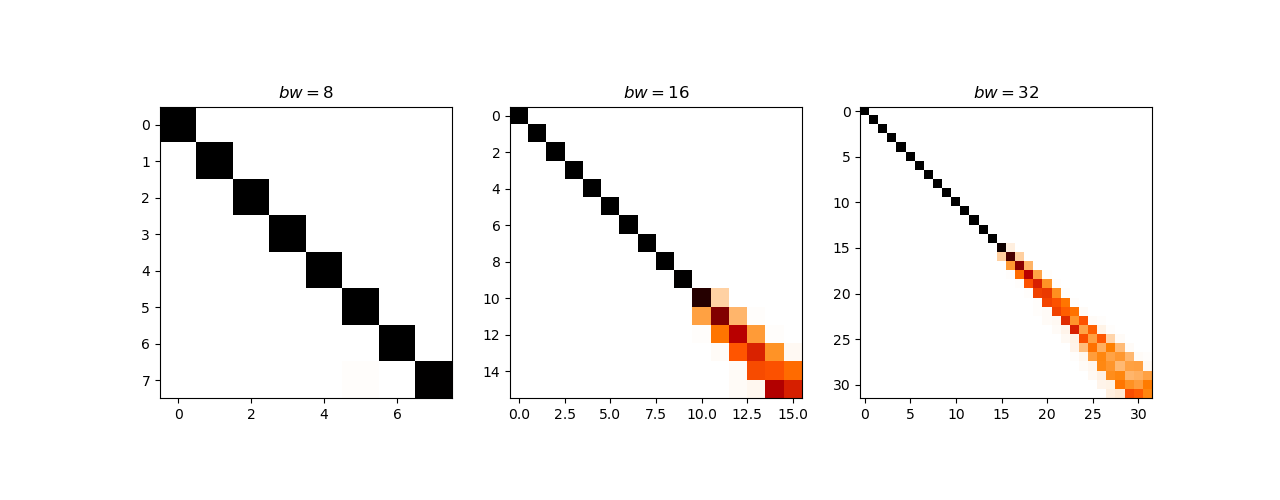
\includegraphics[width=0.9\textwidth]{../codes/03.FEM_laplacian/equiangular/normal/img/linearFEM.png}
	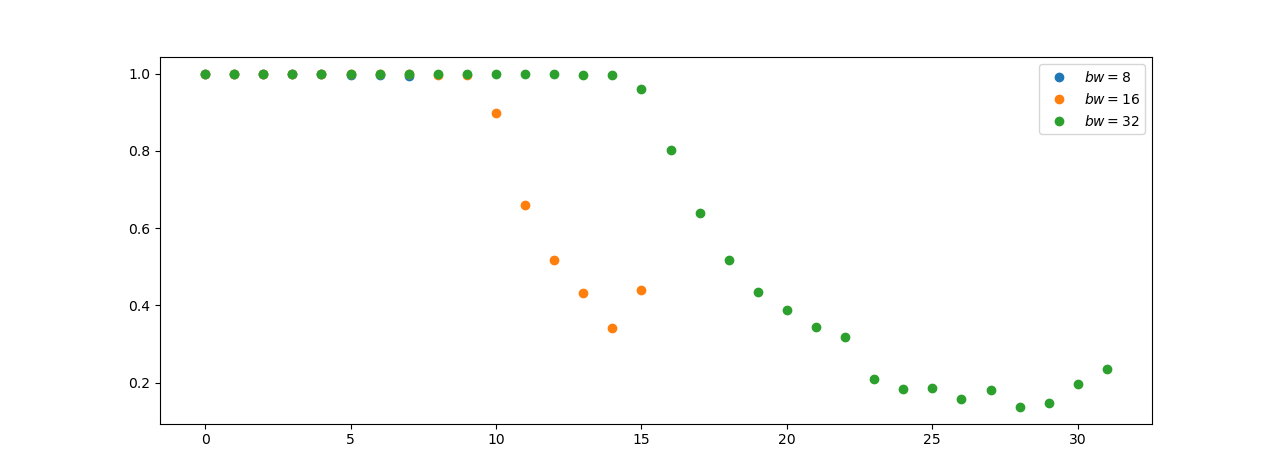
\includegraphics[width=0.9\textwidth]{../codes/03.FEM_laplacian/equiangular/normal/img/linearFEM_diagonal.png}	
	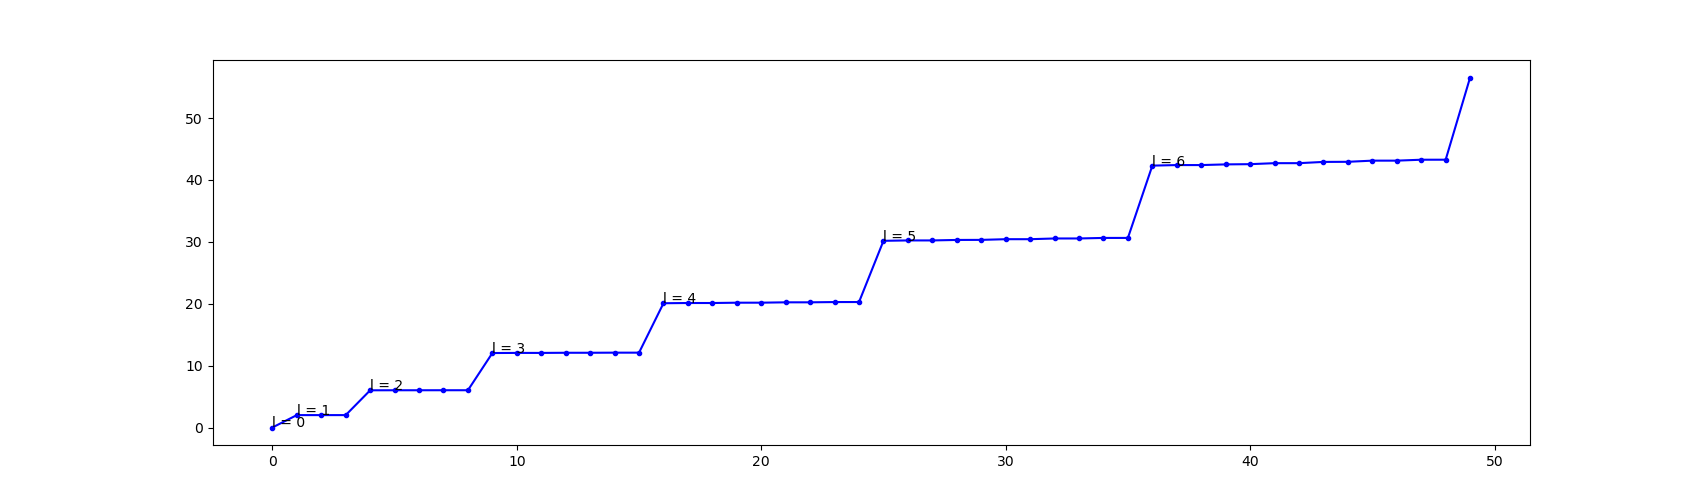
\includegraphics[width=0.9\textwidth]{../codes/03.FEM_laplacian/equiangular/normal/img/FEM_eigenvalues_16.png}	
\end{figure}

\paragraph{Lumping the mass matrix}


\begin{figure}[h]
	\label{fig:FEMequiangularLumped}
	\caption{Lumped Linear FEM Laplacian on equiangular sampling}
	\centering
	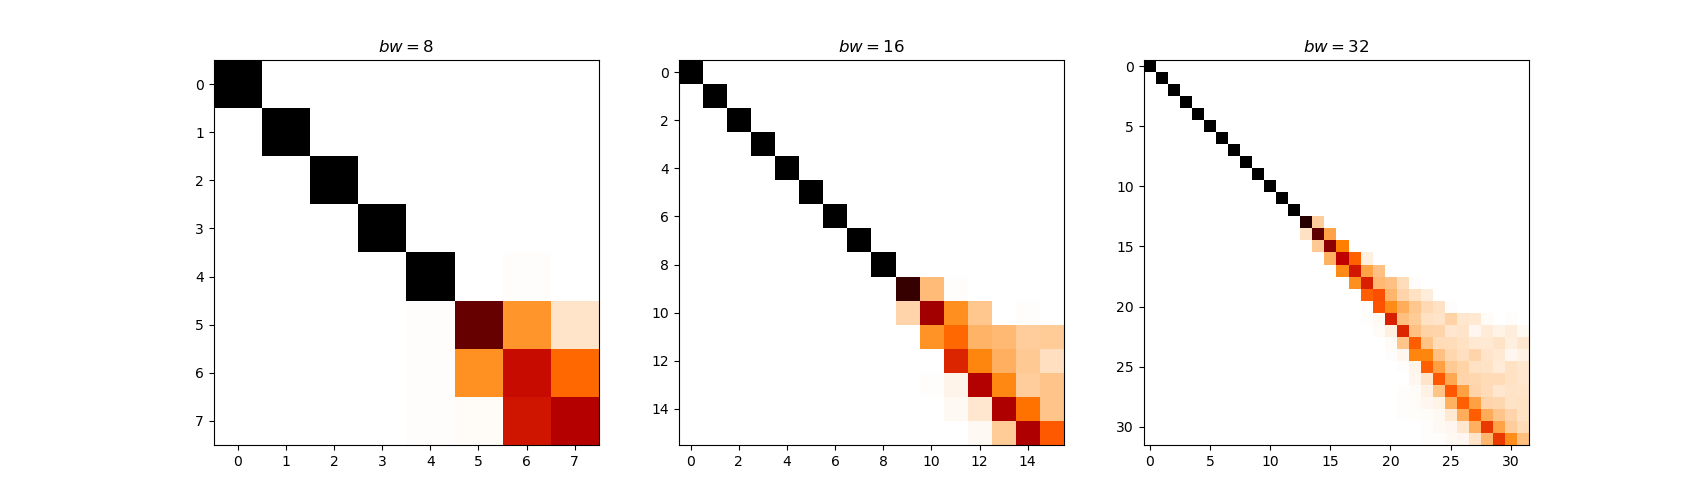
\includegraphics[width=0.9\textwidth]{../codes/03.FEM_laplacian/equiangular/mass_lumping/BL/img/linearFEM.png}
	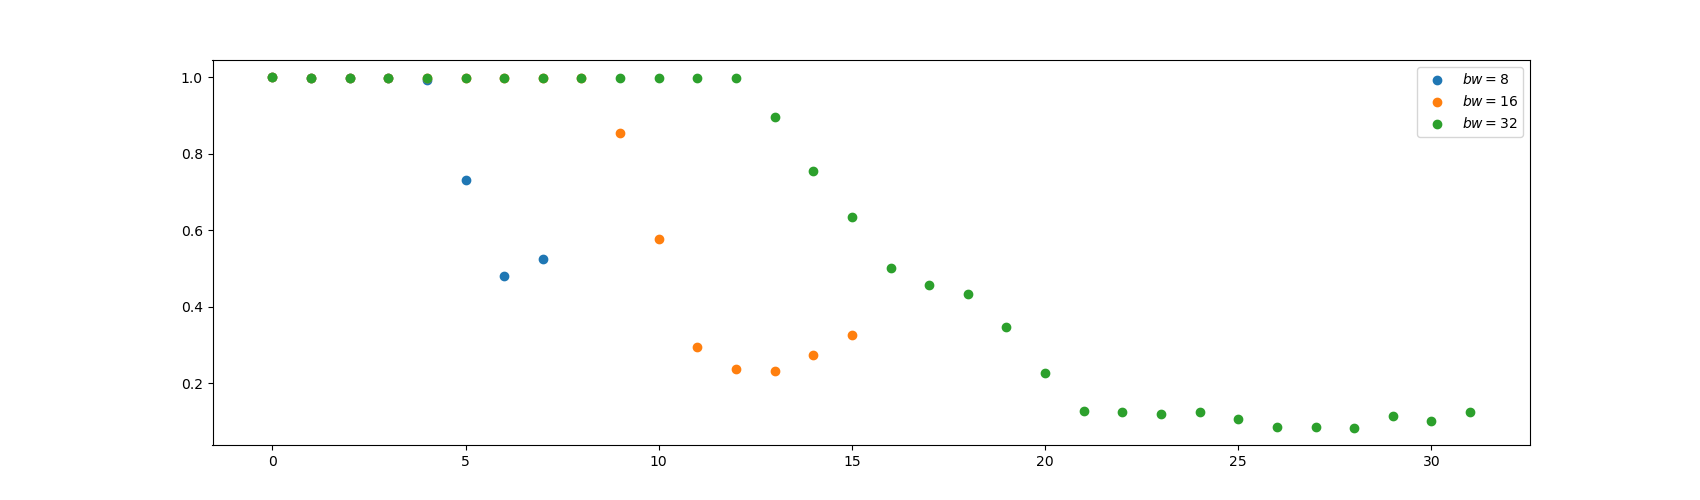
\includegraphics[width=0.9\textwidth]{../codes/03.FEM_laplacian/equiangular/mass_lumping/BL/img/linearFEM_diagonal.png}	
	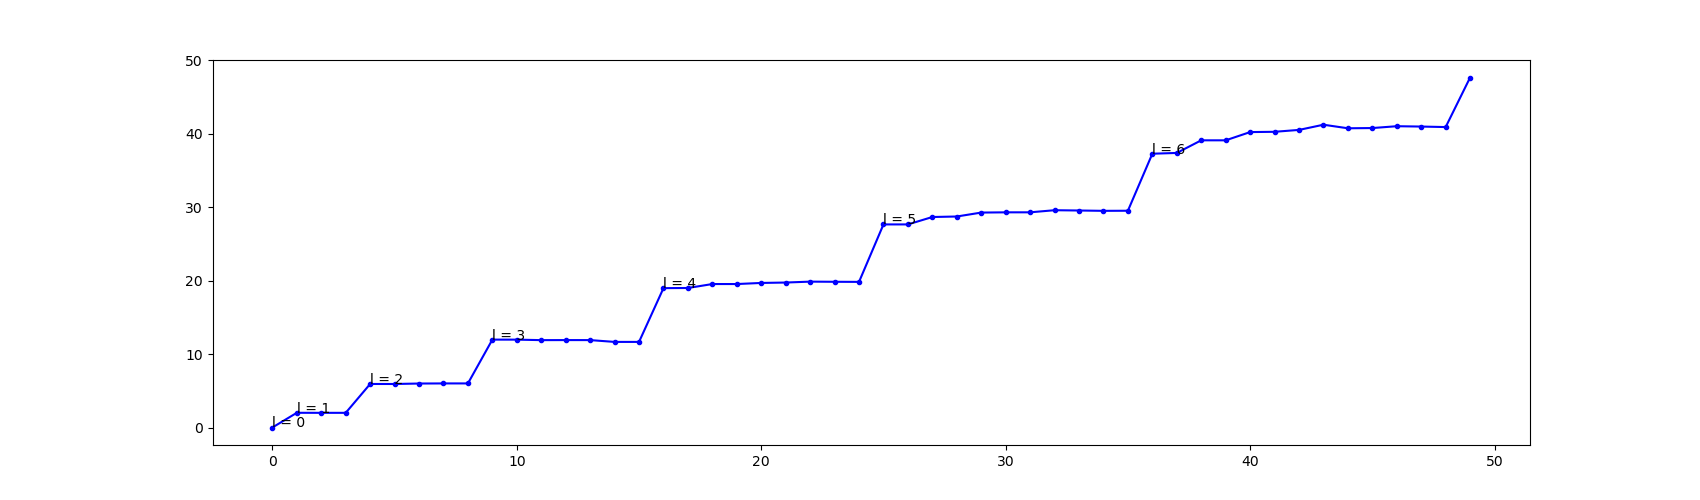
\includegraphics[width=0.9\textwidth]{../codes/03.FEM_laplacian/equiangular/mass_lumping/BL/img/FEM_eigenvalues_32.png}	
\end{figure}

\begin{figure}[h]
	\label{fig:symmetricFEMequiangularLumped}
	\caption{Symmetric Lumped Linear FEM Laplacian on equiangular sampling}
	\centering
	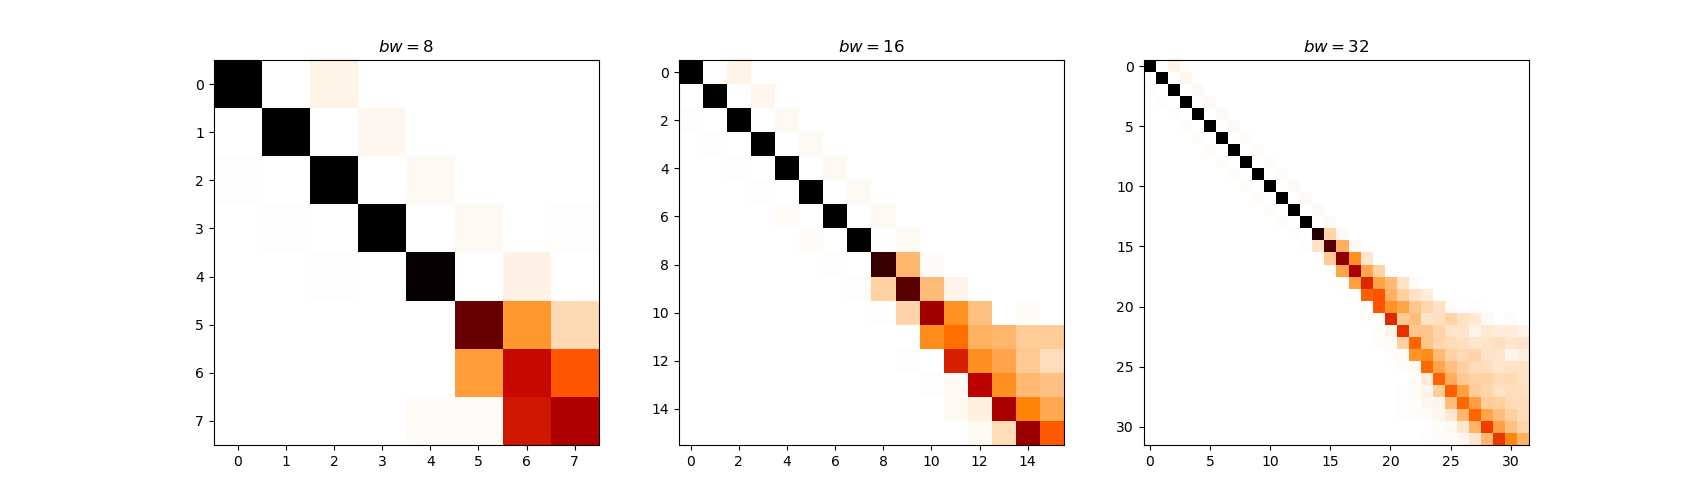
\includegraphics[width=0.9\textwidth]{../codes/03.FEM_laplacian/equiangular/mass_lumping/BLB/img/linearFEM.png}
	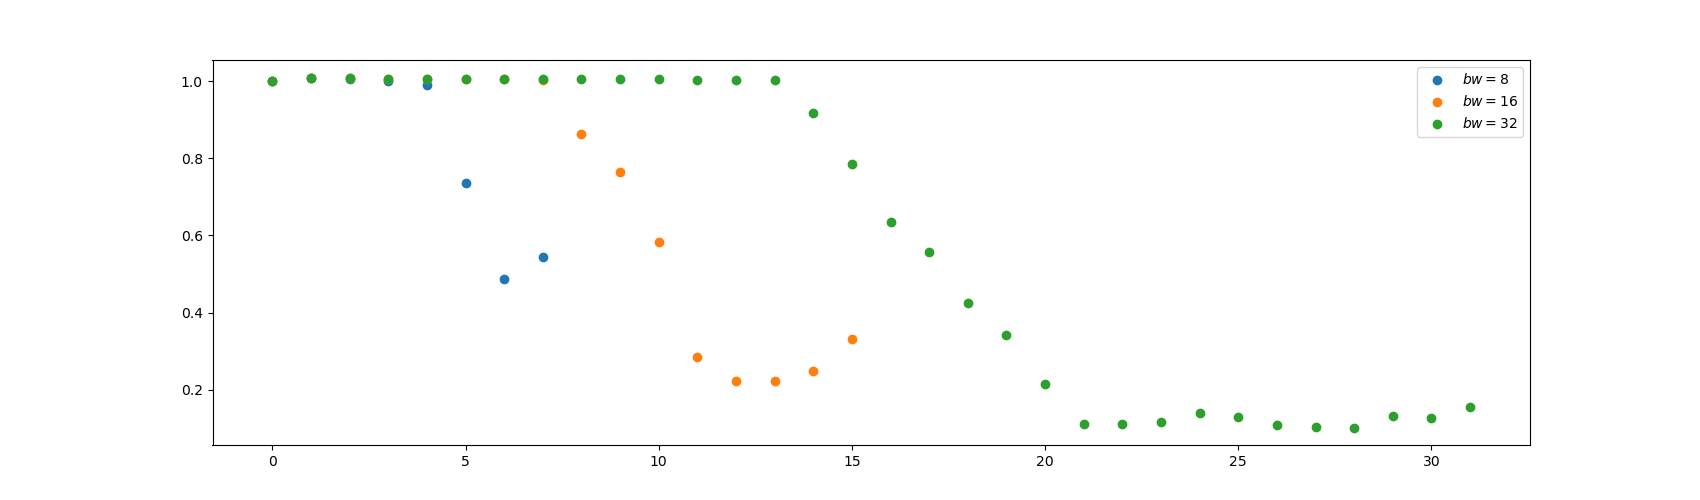
\includegraphics[width=0.9\textwidth]{../codes/03.FEM_laplacian/equiangular/mass_lumping/BLB/img/linearFEM_diagonal.png}	
	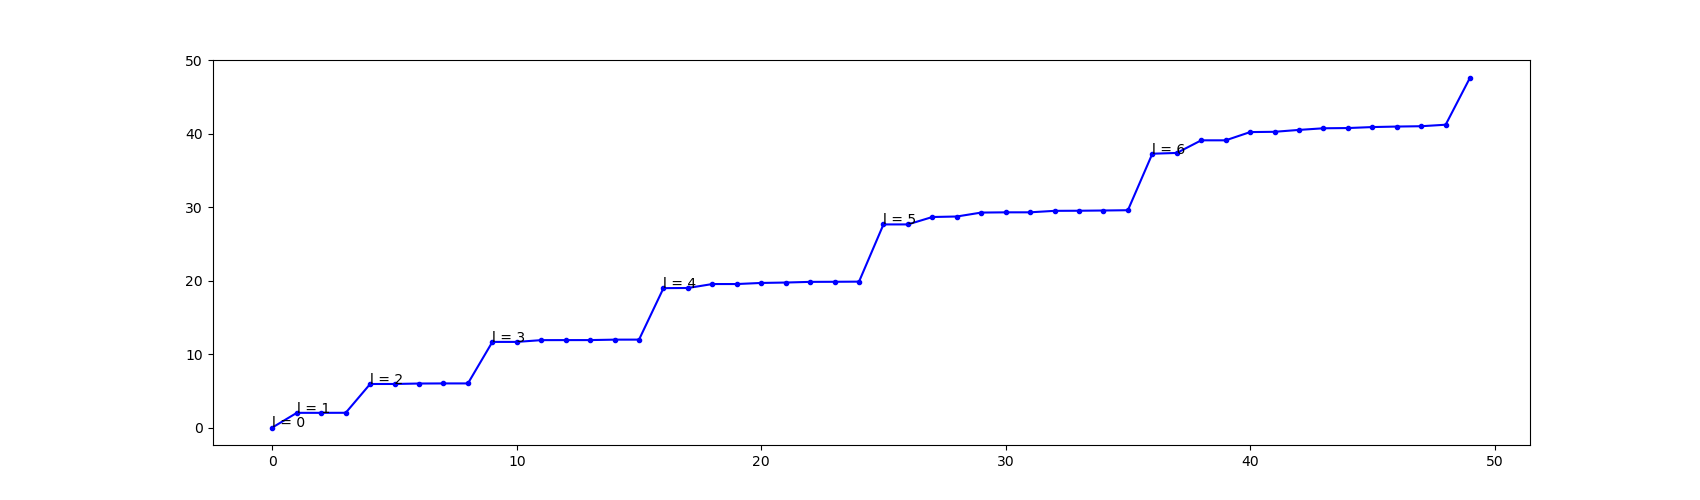
\includegraphics[width=0.9\textwidth]{../codes/03.FEM_laplacian/equiangular/mass_lumping/BLB/img/FEM_eigenvalues_32.png}	
\end{figure}
\subsubsection{Diffusion with the exponential matrix}

\paragraph{HEALPix}
\begin{figure}[h]
	\label{fig:FEM and graph diffusion on HEALPix}
	\caption{linear FEM and HKGL diffusion on HEALPix}
	\centering
	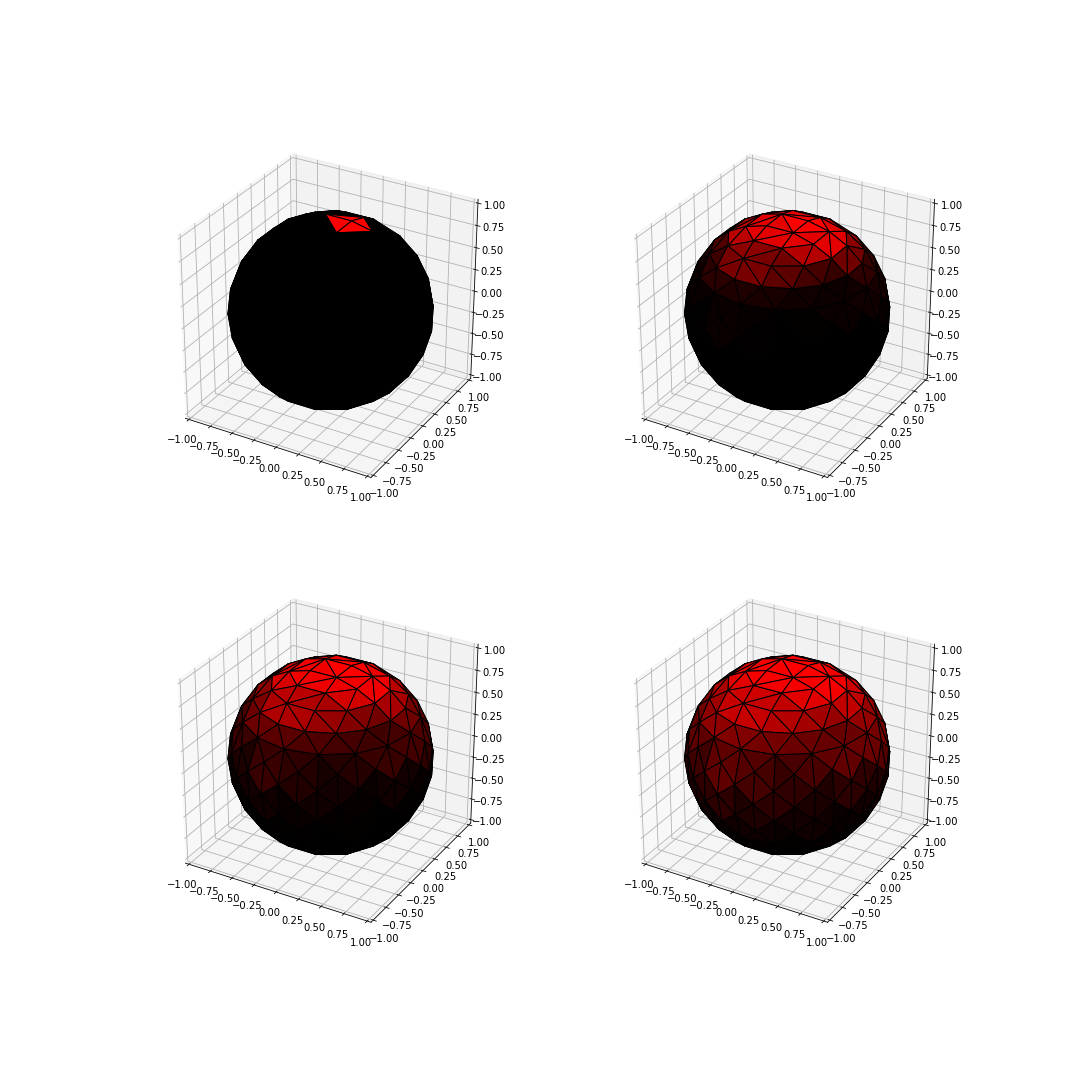
\includegraphics[width=0.6\textwidth]{../codes/03.FEM_laplacian/HEALPix/17_diffusion_img/FEM_diffusion.png}
	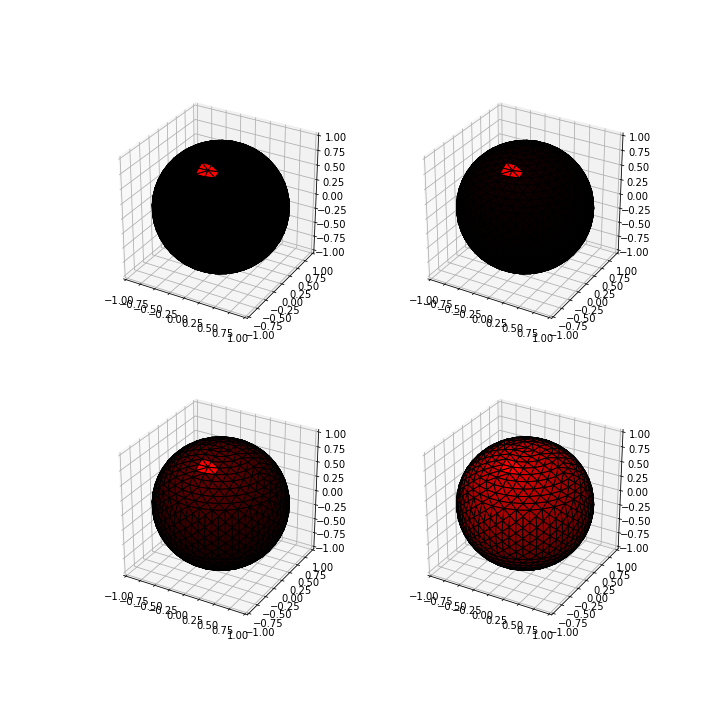
\includegraphics[width=0.6\textwidth]{../codes/03.FEM_laplacian/HEALPix/17_diffusion_img/GRAPH_diffusion.png}	
\end{figure}
\paragraph{Equiangular}
\begin{figure}[h]
	\label{fig:FEM and graph diffusion on equiangular sampling}
	\centering
	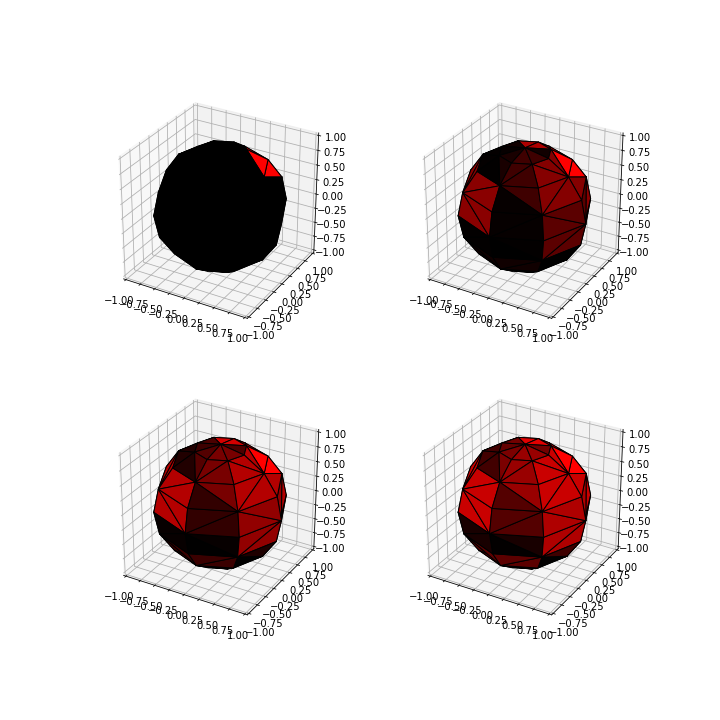
\includegraphics[width=0.6\textwidth]{../codes/03.FEM_laplacian/equiangular/normal/17_diffusion_img/FEM_diffusion.png}
	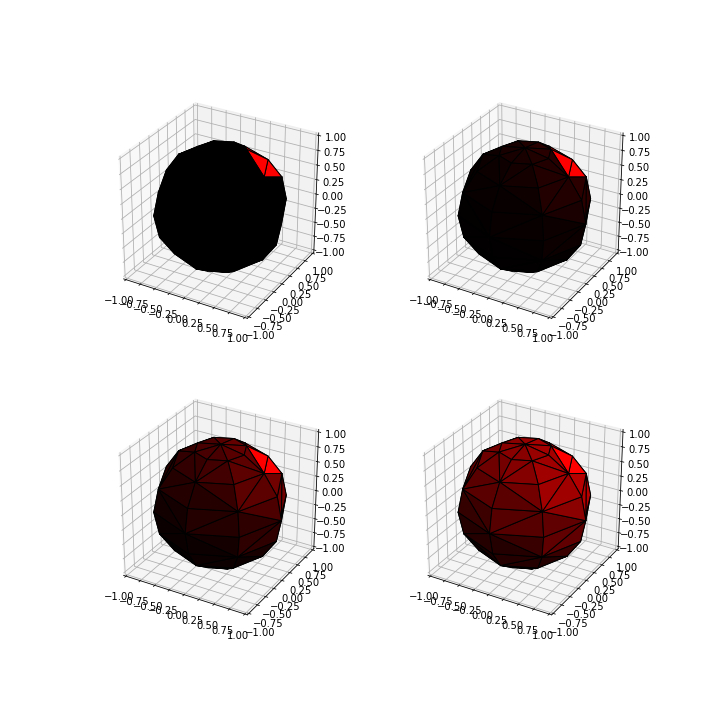
\includegraphics[width=0.6\textwidth]{../codes/03.FEM_laplacian/equiangular/normal/17_diffusion_img/GRAPH_diffusion.png}
	\caption{FEM and HKGL diffusion on equiangular sampling}
\end{figure}
\paragraph{Lumped mass matrix}

\begin{figure}[h]
	\label{fig:FEM diffusion on equiangular sampling}
	\centering
	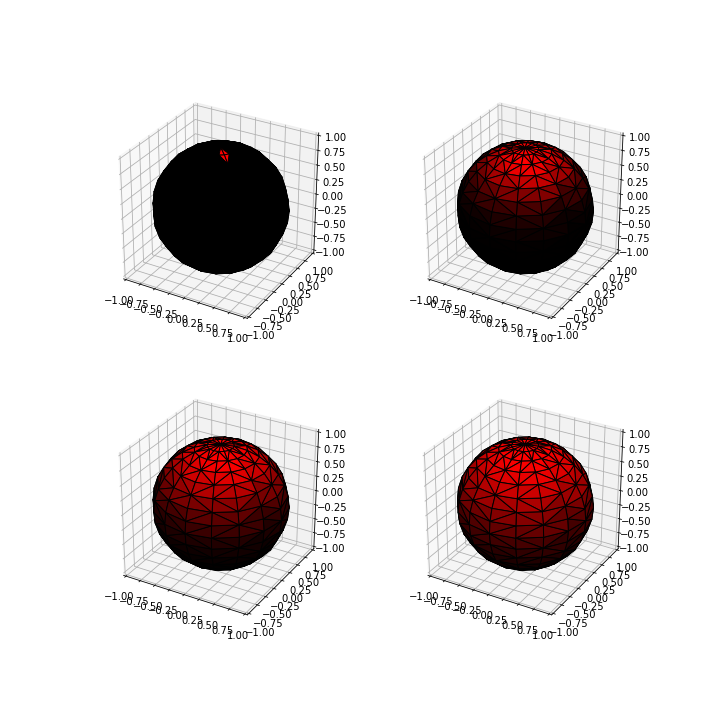
\includegraphics[width=0.4\textwidth]{../codes/03.FEM_laplacian/equiangular/mass_lumping/BL/img/FEM_diffusion.png}
	\caption{ FEM diffusion on equiangular sampling}
\end{figure}
\begin{figure}[h]
	\label{fig:FEM lumped diffusion on equiangular sampling}	
	\centering
	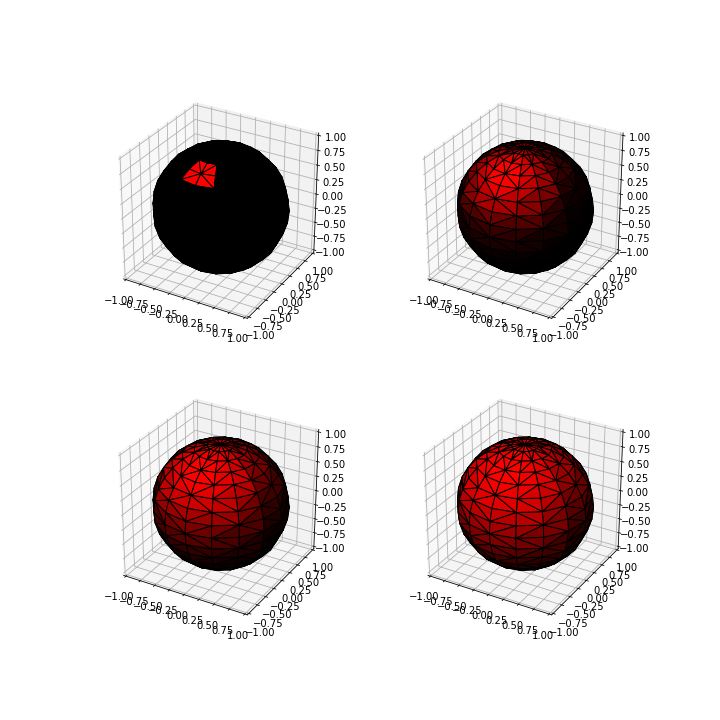
\includegraphics[width=0.4\textwidth]{../codes/03.FEM_laplacian/equiangular/mass_lumping/BL/img/FEM_lumped_diffusion.png}	
	\caption{Lumped FEM diffusion on equiangular sampling}
\end{figure}
\begin{figure}[h]
	\label{fig:FEM lumped symmetric diffusion on equiangular sampling}
	\centering
	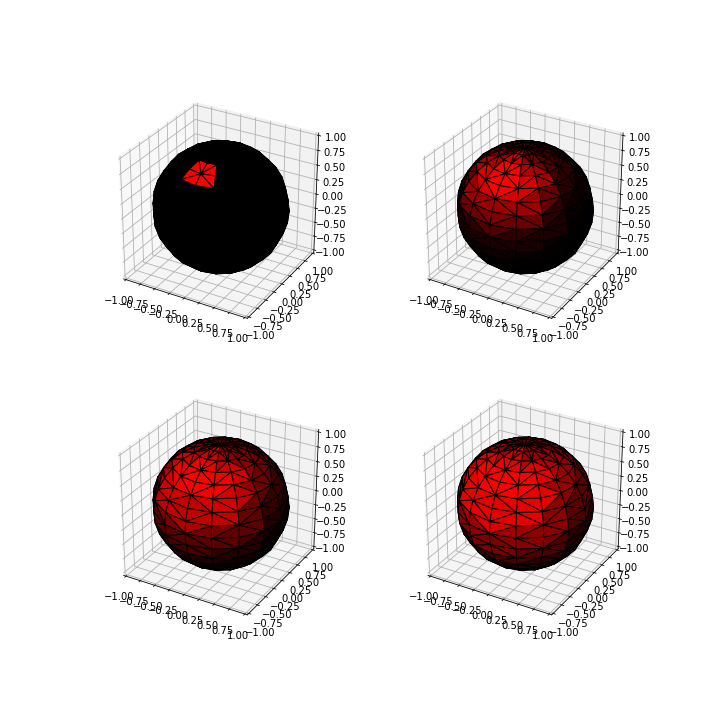
\includegraphics[width=0.4\textwidth]{../codes/03.FEM_laplacian/equiangular/mass_lumping/BL/img/FEM_lumped_symmetric_diffusion.png}
	\caption{Lumped symmetric FEM diffusion on equiangular sampling}
\end{figure}

\subsubsection{Equivariance error}

\begin{figure}[h]
	\label{fig:FEM equivariance error}
	\centering
	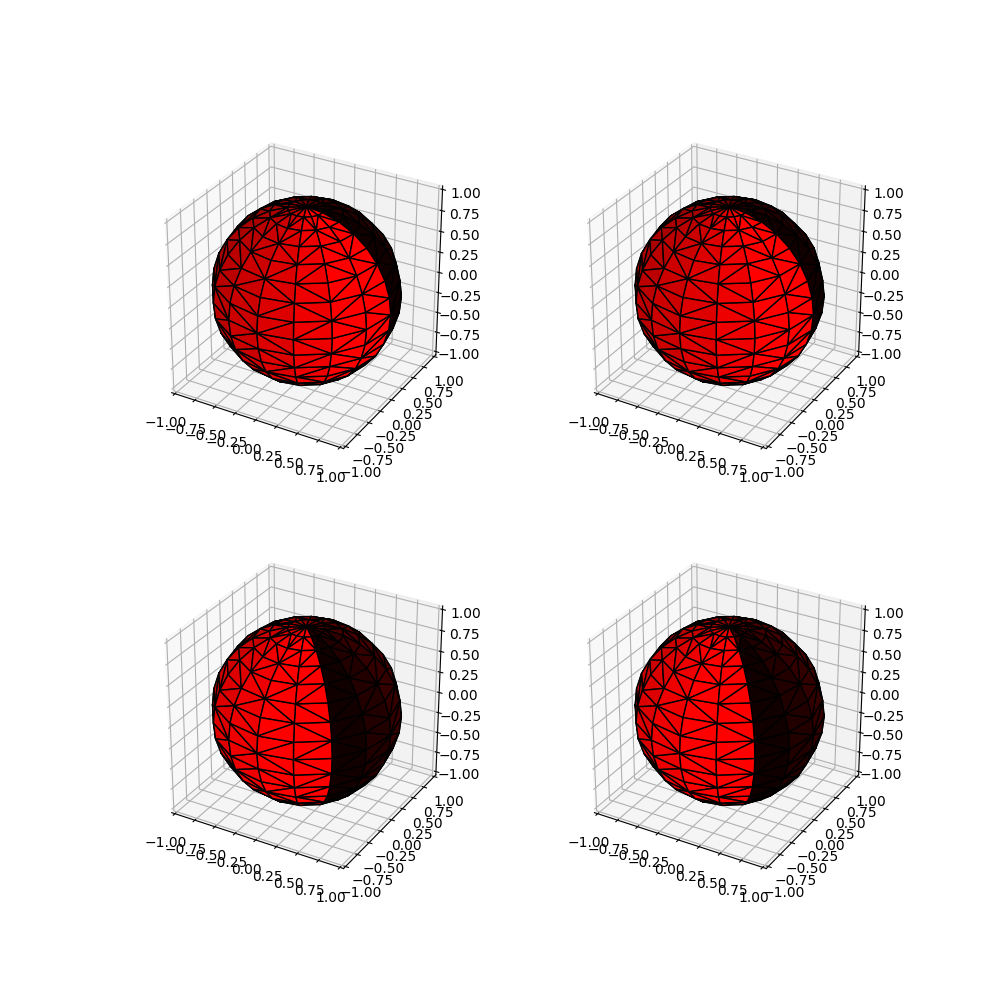
\includegraphics[width=0.6\textwidth]{../codes/03.FEM_laplacian/equiangular/normal/img/equivariance_error_FEM.png}
	\caption{FEM equivariance error}
\end{figure}
\begin{figure}[h]
	\label{fig:GRAPH equivariance error}
	\centering
	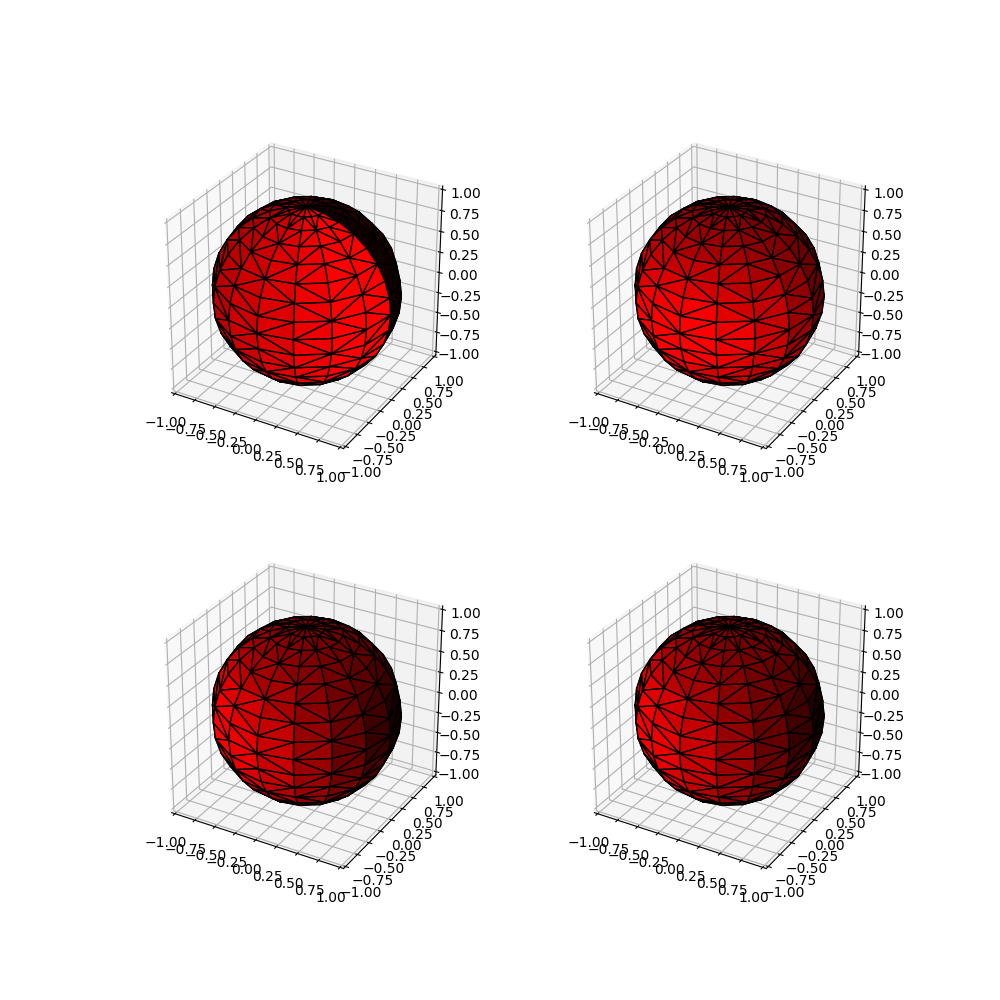
\includegraphics[width=0.6\textwidth]{../codes/03.FEM_laplacian/equiangular/normal/img/equivariance_error_GRAPH.png}
	\caption{Graph equivariance error}
\end{figure}





\pagebreak


%*******************************************************************************
%*********************************** Conclusions ***************************
%*******************************************************************************
%!TEX root = 0.main.tex

\section{Conclusions}\label{sec:Chapter4}




\subsection{Experimental validation: SHREC17}
\label{sec:Chapter5:Experimental validation}
Gusset et al. \cite{Gusset} implemented the graph proposed in this work in a GCNN and three other rotation equivariant neural networks on a popular classification problem \cite{SHREC17}. The four models tested were the following: the original version of DeepSphere, Deepsphere \textit{Optimal} - obtained implementing the thresholding procedure described in this work in section \ref{sec:Chapter2:How to build a good graph} - and the traditional SCNNs of Cohen et al. \cite{SCNN} introduced in section \ref{sec:Chapter1:SCNN} and of Esteves et al. \cite{Esteves}
\paragraph{On the Equiangular sampling}. They compare with two different metrics  (accuracy, F1-score) the performances of these four rotation invariant models, while also comparing the speed of inference and of training of each model. Results are shown in table \ref{tab:SHREC17_class}.  It can be seen how \textit{DeepSphere Optimal} has \textit{always} the highest score between all the rotation equivariant models, no matter the evaluation metric. Furthermore, its performances in terms of speed of inference and training are second only to DeepSphere, remaining by far faster than the other two SCNNs. 
\begin{table}[ht]
	\centering
	\begin{tabular}{l|c c r r r}
		\multicolumn{1}{l}{} & \multicolumn{2}{c}{performance} & \multicolumn{1}{c}{size} & \multicolumn{2}{c}{speed}\\
		\cmidrule(lr){2-3} \cmidrule(lr){4-4} \cmidrule(lr){5-6}
		\multicolumn{1}{l}{Method} & Accuracy & F1-score & params & inference & training \\ \hline
		Cohen \emph{s2cnn\_simple} & 78.59 & 78.85 & 400k & 12ms & 32h\\
		Esteves \emph{sphericalcnn} & 79.18 & 79.36 & 500k & 9.8ms & 2h52\\ \hline
		Deepsphere & 73.36 & 73.67 & 190k & \textbf{0.98ms} & \textbf{43m} \\
		\textbf{Deepsphere \emph{Optimal}} & \textbf{80.42} & \textbf{80.65} & 190k & 1.0ms & 48m
	\end{tabular}
	\caption{Results form \cite{Gusset}. Performances of four rotation equivariant GCNNs and two SCNNs on the popular classification task SHREC17.}
	\label{tab:SHREC17_class}
\end{table}
\paragraph{On HEALPix }
Gusset et al. repeated the same test on the same dataset on a HEALPix sampling with $N_{side}=32$. Results can be seen in table \ref{table:results}.
\begin{table}[h!]
	\centering
	\begin{tabular}{ c|c|c } 
		& DeepSphere & DeepSphere \textit{Optimal} \\ 
		\hline
		accuracy & 82.23\% & 82.76\% \\ 
	\end{tabular}
	\caption{\label{table:results}Results form Gusset et al. Accuracy on the HEALPix sampling}
\end{table}
Being the new graph of DeepSphere Optimal more equivariant to rotations, we expected to see an improvement in the accuracy, as we did in the equiangular case. The fact that this improvement was not observed on HEALPix means that, in this case, the original DeepSphere graph $W$ \textit{is already sufficiently equivariant to rotations}. By this we mean that for this task, being equivariant to rotations of the low frequency eigenmodes is sufficient to obtain good results, and that being rotation equivariant to the higher frequencies does not lead to any improvement.

\subsection{Confront of different Discrete Laplacians on the equiangular sampling}
We conclude by showing how the different discrete Laplacians $\mathbf L$ illustrated so far compare in terms of equivariance error and computational time of the filter $\mathcal F(\mathbf f) = \mathbf L\mathbf f$. We can see how the three sparse discrete Laplacians are one order of magnitude faster than the two full Laplacians. The FEM approach is actually able to reduce the equivariance error compared to the HKGL, and it stays low even when using the sparse, lumped approximation $B^{-1}A$. The lumped FEM Laplacian $D^{-1}A$ performs really well, and gets close to the performances of the graph Laplacian of Khasanova and Frossard. 
\begin{figure}[h!]
	\centering
	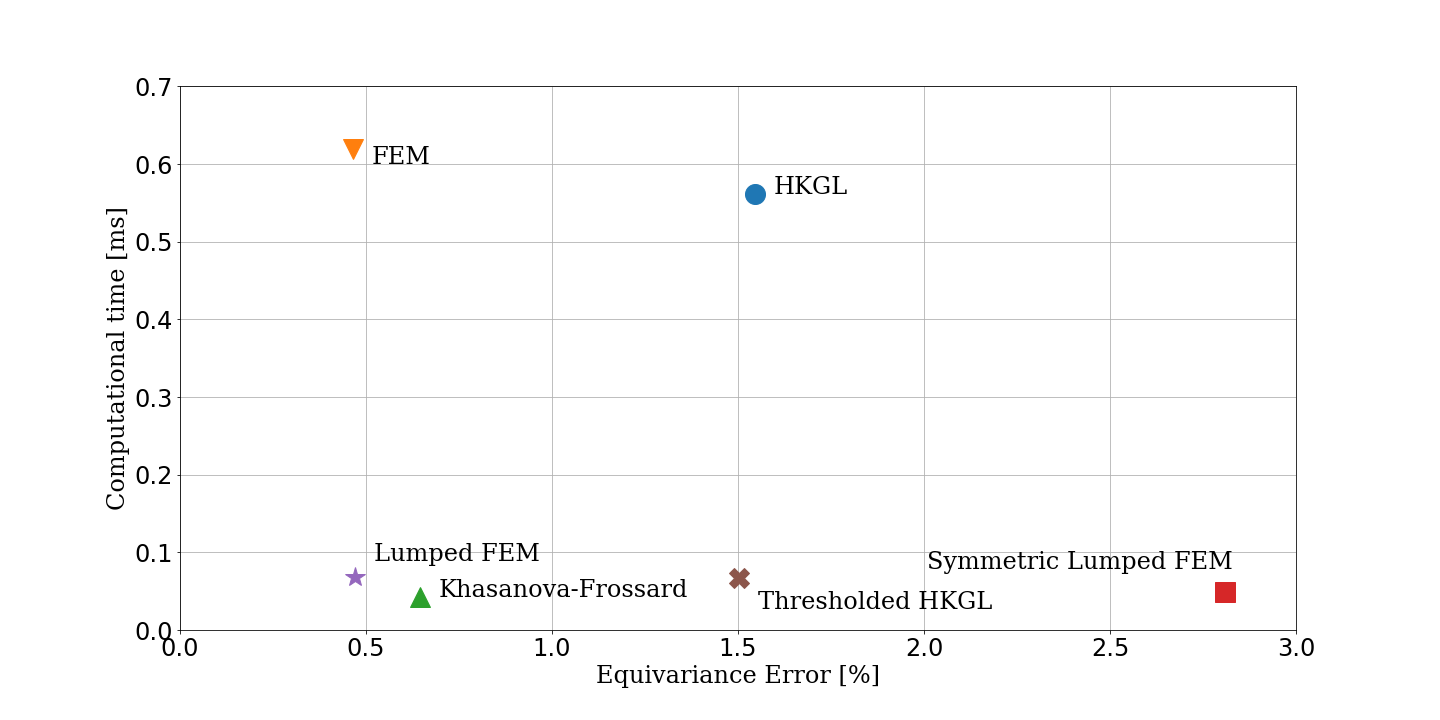
\includegraphics[width=\textwidth]{../codes/06.Equivariance_error/tradeoff.png}
	\caption{\label{fig:tradeoff}Trade-off between computational time and equivariance error for the filter $\mathbf L$ for different discrete Laplacians on the equiangular sampling}
\end{figure}

\subsection{Final considerations and future work}


Having a metric means using a \textit{non-symmetric matrix} $B^{-1}A$ such that the generalized eigenvalue problem $Av = \lambda B v$ is such that $v_i$ approximates the corresponding sampled SH and $VBV^T=I$. With a graph this is not possible since we restrict ourself to \textit{symmetric} Laplacians and thus make it impossible to incorporate a metric $B$, since the symmetry of $L$ imposes $VV^T=I$. However, there are good approximations that even by being symmetric perform well: the Khasanova-Frossard graph is an example. Further research would be 


\pagebreak
{\small \bibliography{references.bib}} 
\nocite{*}
\pagebreak

\pagebreak
\null
\newpage
\section{Appendix}

In this section we provide the necessary definitions and mathematical concepts necessary to properly introduce the weak formulation of a differential problem, the Galerkin method and finally the Finite Element Method.\\

\paragraph{Linear operators, functionals and bilinear forms} A \textit{linear operator} $L: X\to X$ from the Hilbert space $(X, \norm \cdot)$ to itself is a map such that $L(\alpha x + \beta y) = \alpha L x + \beta L y$. A linear operator on a Hilbert space is \textit{continuous} (or {bounded}) if $\exists M:\ |Lx|\leq Mx$. $(x, \lambda)$ are called respectively \textit{eigenvector} and \textit{eigenvalue} of the linear operator $L$ if the image of $x$ through $L$ is a rescaling of $x$ of factor $\lambda$ i.e. $Lx = \lambda x$. The operator $L$ is called \textit{self-adjoint} if $\langle Lx, y\rangle = \langle x,Ly\rangle\ \  \forall x,y \in X$. Self-adjoint operators have two important properties: their eigenvalues are real, and two eigenvectors $x, y$ associated to different eigenvalues $\lambda, \mu$ are orthogonal. Indeed 
\begin{align*}
	\langle Lx, y\rangle &= \langle x,Ly\rangle,\\
	\langle \lambda x, y\rangle &= \langle x,\mu y\rangle,\\
	\lambda \langle  x, y\rangle &= \mu \langle x, y\rangle,
\end{align*}
that implies $ \langle  x, y\rangle = 0$. If the eigenvectors of a self-adjoint operator $L$ span the whole space $X$, then $L$ is called \textit{diagonalisable}.  A linear operator from a Hilbert space $X$ to $\mathbb R$ is called a linear \textit{functional} on $X$. A functional is bounded if $\exists M\geq 0: \ |Lx|\leq M\norm x$. The normed vector space made by the set of all linear bounded functionals on $X$ endowed with the norm $\norm L = sup_{v\in X}|Lv|/\norm v$ is called the \textit{dual} space of $X$ and is indicated with $X^\star$. An important property of linear functionals is that for every functional $L\in X^\star$, there exists a unique vector $u\in X$ such that
$$Lv = \langle u, v\rangle\quad \forall v\in X$$ 

A \textit{bilinear form} on the vector space $X$ is a map $a(\cdot, \cdot): X\times X\to F$ that is linear with respect to both arguments. It is said to be \textit{strongly coercive} if \\
$\exists\alpha>0:\ |a(x, x)|\geq \alpha \norm {x}^2$, and \textit{bounded} if $\exists M>0:\ |a(x, y)|\leq M \norm x \norm y$.

\paragraph{The Lax-Milgram theorem}
Before introducing the Galerkin method the last thing to do is to state the Lax-Milgram theorem, theorem that is the foundation of the FEM formulation.
\vspace{0.5cm}
\begin{theorem}[Lax-Milgram]
	If \(a(\cdot, \cdot)\) is a bounded and strongly coercive bilinear form on the Hilbert space \(X\),  $L\in X^\star$ is a linear bounded functional on $X$, there exist a unique solution $f$ to the following problem:
	\begin{equation}\label{eq:variational abstract problem}
	\text{Find }f\in X\text{ such that } a(f, v)=Lv \text{ for all } v \in X
	\end{equation}
	For such \(f\) one has \(\|f\| \leq \frac{1}{\alpha}\norm L\) where \(\alpha>0\) is the coercive constant \\\(a(v, v) \geq \alpha\norm v^{2} \forall v \in X.\)
\end{theorem} 
\vspace{0.5cm}
The Finite Element Method takes a PDE problem in strong form (\ref{eq:strong form}), reformulates it in the equivalent \textit{weak form} (\ref{eq:variational abstract problem}) through suitable definitions of $X, a(\cdot, \cdot), L$ and finally solves it through polynomial interpolation.
\subsubsection{Weak formulation of a PDE and Galerkin Method}

Galerkin's method is a method to approximate the solution $f$ of an infinite dimensional problem of the form (\ref{eq:variational abstract problem}) with the solution $f_h$ of a finite dimensional problem. Our goal is now to explain how to write a differential problem like 
\begin{align}\label{eq:strong form}
\begin{split}
&\text{Given a regular domain }\Omega\subset\mathbb R^2\text{ and } u\in C(\Omega)\text{, find }f\in C^2(\Omega) \text{ such that}\\
&\begin{cases}
-\partial_{x_1x_1}f(\mathbf x) - \partial_{x_2x_2}f(\mathbf x) = u(\mathbf x) & \mathbf x \in \Omega\\
f(\mathbf x) =  0& \mathbf x \in \partial \Omega
\end{cases}
\end{split}
\end{align}
in the form \ref{eq:variational abstract problem}. Let's multiply the differential equation times a sufficiently regular function $v$ that vanishes on $\partial \Omega$ and integrate on $\Omega$. We obtain
\begin{align}
\begin{cases}
-\int_{\mathbb S^2}\Delta f(\mathbf x)v(\mathbf x)d\mathbf x =\int_{\mathbb S^2} u(\mathbf x)v(\mathbf x)d\mathbf x &\quad \mathbf x \in \Omega\\
f(\mathbf x) =  0&\quad \mathbf x \in \partial \Omega
\end{cases}	
\end{align}
 Since the contribution of both $f$ and $v$ on the border $\partial \Omega$ is zero, \\$\int_{\partial \Omega}\nabla f \cdot \mathbf nv d\sigma=0$ and integrating by parts we get

\begin{equation}\label{eq:int by parts}
	\int_\Omega \nabla f(\mathbf x)\cdot\nabla v(\mathbf x) d\mathbf x = \int_\Omega  u(\mathbf x)\cdot v(\mathbf x)d\mathbf x
\end{equation}

By defining $a(f, v):=	\int_\Omega \nabla f(\mathbf x)\cdot\nabla v(\mathbf x) d\mathbf x $ and $Lv := \int_\Omega  u(\mathbf x)\cdot v(\mathbf x)d\mathbf x$ problem \ref{eq:int by parts} can be written in the form of equation \ref{eq:variational abstract problem}. It remains to choose a Hilbert space $(X, \langle\cdot,\cdot\rangle_X)$ such that (i) $X$ is "big enough" to include those functions such that all the integrals and derivatives in the problem \ref{eq:int by parts} is well defined. This means that $X$ must include those functions $f$ such that $f, \nabla f$ are in $L^2(\Omega)$ and has to be \textit{complete} with respect to the norm induced by the scalar product $\langle\cdot,\cdot\rangle_X$. At the same time $X$ must be (ii) "small enough" to include only those functions that vanish on the boundary of $\Omega$. and (iii) the hypothesis of the Lax-Milgram theorem are satisfied, i.e. $a(\cdot, \cdot)$ is actually bounded and coercive and $L$ is bounded and linear. It turns out that such an Hilbert space exists: it is called $H^1_0(\Omega)$, it contains all the functions $v$ such that $v\in L^2(\Omega), \nabla v\in L^2(\Omega)$ and it is endowed with the scalar product 
$$
\langle u, v\rangle_{H^1_0(\Omega)} = \int_\Omega u(\mathbf x)v(\mathbf x)d\mathbf x + \int_\Omega\nabla u(\mathbf x)\cdot \nabla v(\mathbf x) d\mathbf x
$$
$H^1_0$ contains only those functions that vanish on $\delta \Omega$ i.e. \\$f\in H^1_0(\Omega)\cap C(\Omega) \implies \left.f(\mathbf x)\right|_{\partial\Omega}=0$. This means that thanks to Lax-Milgram theorem the problem

\begin{equation}\label{eq:final variational form}
\begin{split}
	&\text{Given }u\in L^2(\Omega)\text{ find }f\in H^1_0(\Omega)\text{ such that }\\
	&\int_\Omega \nabla f(\mathbf x)\cdot\nabla v(\mathbf x) d\mathbf x = \int_\Omega  u(\mathbf x)\cdot v(\mathbf x)d\mathbf x\quad \forall v\in H^1_0(\Omega)
\end{split}
\end{equation}

\textit{has one and only one solution in} $H^1_0(\Omega)$. However, to have this result (existence and uniqueness of the solution) we had to pay the price of looking for the solution $f$ in $H^1_0(\Omega)$, a much bigger space than  $C^2(\Omega)$ that we had in the original, strong form of the problem. This means that our solution $f\in H^1_0(\Omega)$ to the problem (\ref{eq:final variational form}) could not be a solution to problem (\ref{eq:strong form}), because it could be not regular enough and the second derivative $\Delta f$ could not exist! Fortunately there are regularity results - that we omit here - that assure that if the forcing term $u$ is regular enough, then also the solution $f$ will be regular and thus the two formulations - strong and weak - of the problem are actually equivalent, and thus solving \ref{eq:final variational form} eventually leads to solving \ref{eq:strong form}.

Now that we know that a solution exists, we need to compute it! Computing it analytically is often impossible; Galerkin's method in a mathematical tool provide us a way to compute an approximation of the solution $f$. Take the weak problem \ref{eq:variational abstract problem}, but restrict the ambient space to be a finite dimensional subspace of $X$, say $V_h = \text{span}\{\phi_0, ..., \phi_{n-1}\}$. We write thus the Galerkin problem
\vspace{0.5cm}

\begin{equation}\label{eq:Galerkin problem}
		\text{Find }f_h\in V_h\text{ such that } a(f_h, v_h)=\langle u_h, v_h\rangle \text{ for all } u_h \in V_h
\end{equation}
\vspace{0.5cm}

The key property of the Galerkin method is that the error $f-f_h$ is orthogonal to $V_h$; thus by choosing a sequence of finite dimensional spaces that fill the original space $X$, we can get as close as we want to the continuous solution $f$.
To solve equation \ref{eq:Galerkin problem} we write $f_h, u_h, v$ as linear combinations of the basis $\{\phi_0, ..., \phi_{n-1}\}$
\begin{equation}\label{eq:basis functions}
	\begin{cases}
	f_h = f_0\phi_0 +  f_1\phi_1 + ...  f_{n-1}\phi_{n-1}\\
	u_h = u_0\phi_0 +  u_1\phi_1 + ...  u_{n-1}\phi_{n-1}\\
	v_h = v_0\phi_0 +  v_1\phi_1 + ...  v_{n-1}\phi_{n-1}
	\end{cases}
\end{equation}
 thus obtaining by linearity of the bilinear form and of the scalar product a linear system of equations in the $n$ coordinates of $f_h$
\begin{equation}\label{eq:Galerkin problem in the basis functions}
\text{Find }\mathbf f\in\mathbb R^n\text{ such that } \sum_{j=0}^{n-1}a(\phi_i, \phi_j)f_j=\sum_{j=0}^{n-1}\langle \phi_i, \phi_j\rangle u_j \text{ for all } i=0, ... n-1
\end{equation}

Defining the \textit{stiffness matrix} $(A)_{ij} = a(\phi_i, \phi_j)$ and the \textit{mass matrix} \\$(B)_{ij} = \langle \phi_i, \phi_j\rangle$ we can rewrite problem \ref{eq:Galerkin problem in the basis functions} in the following algebraic form
\begin{equation}\label{eq:Galerkin algebraic}
\text{Find }\mathbf f\in\mathbb R^n\text{ such that } A\mathbf f = B \mathbf u
\end{equation}
where $\mathbf f, \mathbf u$ are the vectors of coordinates of $f_h, u_h$ with respect to the basis $(\phi_i)$. 
\vspace{0.5cm}
\begin{remark}
	 If the basis functions $\phi_i$ are orthonormal, then the mass matrix $B$ is the identity matrix. Furthermore, the scalar product in the space $V_h$ of two functions $u_h, v_h$ is equal to the dot product defined by the mass matrix $B$ in $\mathbb R^n$ of the coordinate vectors
	\begin{equation}\label{eq:dot product}
	\langle u_h, v_h\rangle = \mathbf u^\intercal B \mathbf v
	\end{equation}
	The Galerkin method \ref{eq:Galerkin problem} is well posed by a straight-forward application of the Lax-Milgram theorem, and thus also the system \ref{eq:Galerkin algebraic} admits one and only one solution.
\end{remark}

 \subsubsection{The Finite Element Method}
 
  The Finite Element Method is a technique that let us construct a particular subspace $V_h$ in (\ref{eq:Galerkin problem}) through polynomial interpolation. Let's refer again to the problem \ref{eq:strong form} defined on the domain $\Omega\subset\mathbb R^2$ in figure \ref{fig:omega and mesh}. 
 \paragraph{Approximation of the domain $\Omega$}
\begin{figure}[h]
	\centering
	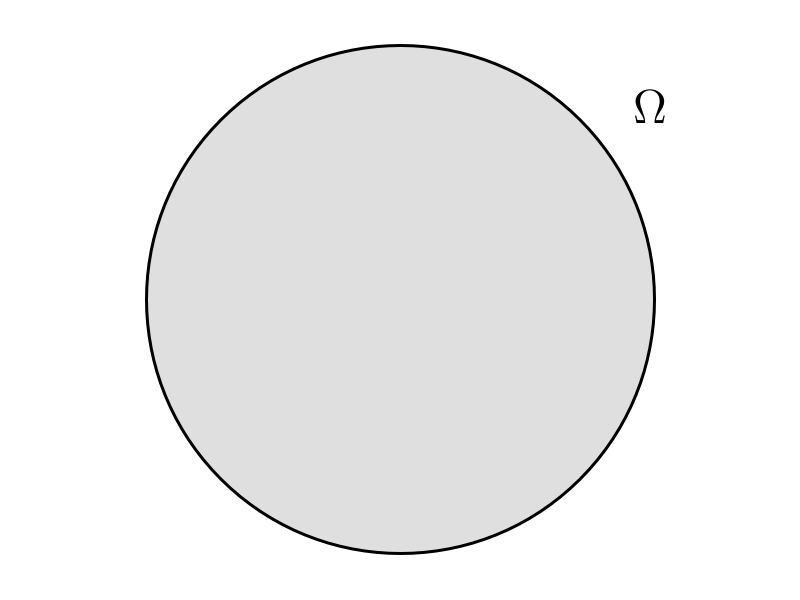
\includegraphics[width=0.4\textwidth]{figs/Chapter3/omega.png}
	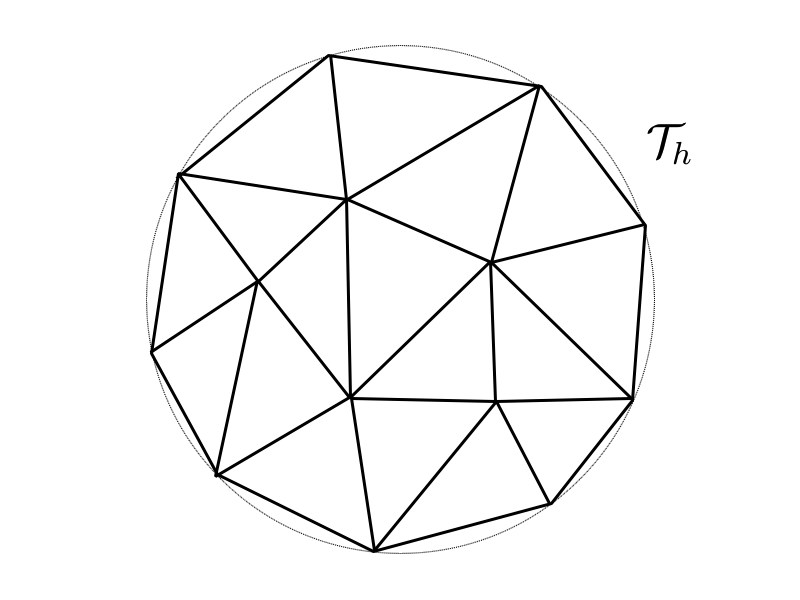
\includegraphics[width=0.4\textwidth]{figs/Chapter3/mesh.png}
	\caption{\label{fig:omega and mesh}The domain $\Omega$ and its approximation $\mathcal T_h$}
\end{figure}
First we need to construct a discretization of the continuous domain $\Omega$. In this example we take the triangulation in figure \ref{fig:omega and mesh} $\mathcal T_h = \left\{\tau_{k} : 1 \leq k \leq q\right\}$, where $h\in\mathbb R$ is a parameter such that every edge of the triangles $\tau_k\in\mathcal T_h$ is smaller than $h$. $\mathcal T_h$ is such that 
\begin{itemize}
	\item The elements \(\tau \in \mathcal{T}_h\) are closed subsets of \(\Omega\) with pairwise disjoint interior and \({\Omega}_h=\bigcup_{\tau \in \mathcal{T}_h} \tau\)
	\item The triangulation \(\mathcal{T}_h\) has no hanging vertices.
\end{itemize}

It's clear that by discretizing the continuous domain $\Omega$ we introduce a first source of errors in the method; however for simplicity we won't take this into account in the next discussion, and we will identify the domain $\Omega$ with the domain $\Omega_h$ covered by $\mathcal T_h$. The quality of the \textit{mesh} $\mathcal T_h$ is important for a good solution; a good quality mesh should avoid triangles with extreme angles and every triangle of $\mathcal T_h$ should look like as much as possible to an equilateral triangle. In figure \ref{fig:bad mesh} we see an example of a bad quality mesh: its triangles look very stretched; there are vertices that are shared by many triangles and vertices that are shared by very few. In figure \ref{fig:omega and mesh} we see a better mesh: there are no stretched triangles, and every vertex is shared by an almost constant number of triangles.
\begin{wrapfigure}{r}{0.3\textwidth}
	\begin{center}
		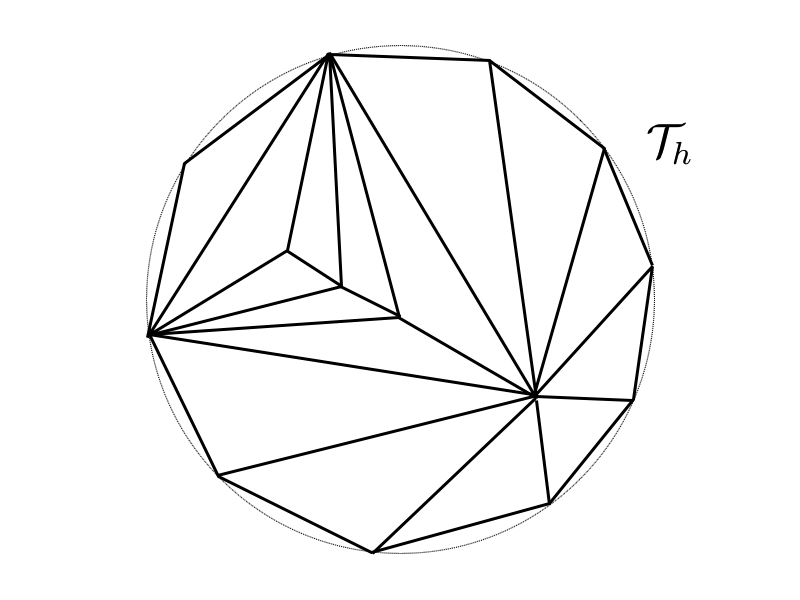
\includegraphics[width=0.4\textwidth]{figs/Chapter3/badmesh.png}
		\caption{\label{fig:bad mesh}A bad quality mesh}
	\end{center}
	
\end{wrapfigure}
\paragraph{Choosing $V_h$ and the basis functions $\phi_i$}

Beyond $X_h^1$, explained in section \ref{sec:Chapter3:FEM on the sphere}, other choices for $V_h$ are possible. A common choice is the space $X_h^{2}$ that is the space of all the piecewise second-order polynomials. In this case, since every second order polynomial in $\mathbb R^2$ has 6 degrees of freedom per each triangle $\tau_k$, meaning that we need to know its values in at least 6 different points on the triangle $\tau_k$ to uniquely identify it, the dimension of the space will grow (figure \ref{fig:elements}). A bigger space means that the approximation $f_h$ will be better, but we'll need more basis functions to define and thus it will result in a bigger linear system $Af = Bu$ and higher computational costs.
\begin{figure}[h!]
	\begin{center}
		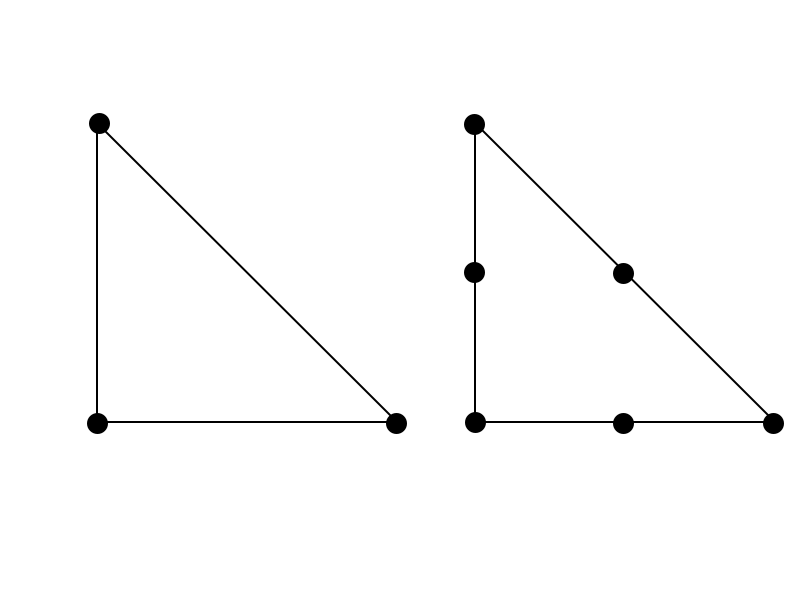
\includegraphics[width=0.4\textwidth]{figs/Chapter3/elemntsP1P2.png}
	\end{center}
	\caption{\label{fig:elements}The degrees of freedom (DOF) for $X_h^{1}$ and $X_h^{2}$ on a reference triangle}
\end{figure}
\paragraph{Assembling the stiffness and mass matrices}
Once defined the basis functions $\phi_i$, the FEM method constructs the stiffness matrix and the mass matrix $(A)_{ij} = a(\phi_i, \phi_j),\  (B)_{ij}=\langle\phi_i,\phi_j\rangle$ and solves the linear system \ref{eq:Galerkin algebraic} for the coefficients $f_i$ of the FEM solution $f_h$. An important fact to notice is both matrices $A$ and $B$ are \textit{sparse} and share the same sparsity pattern. Due to the form of the basis function $\phi_i$, the element $(i, j)$ of these matrices is different from zero only if the supports of the corresponding basis functions $(\phi_i, \phi_j)$ overlap, meaning that the vertices $(x_i, x_j)$ are connected by an edge of the mesh $\mathcal T_h$. In other words, the number of non-null entries of the $i-th$ row of $A$ and $B$ is equal to number of triangles of the mesh $\mathcal T_h$ that share the $i$th vertex i.e., the degree of the $i-th$ vertex.

\paragraph{About the boundary conditions}
	Note that the Dirichlet boundary conditions in the strong formulation of the differential problem \ref{eq:strong form} got transformed in the weak formulation \ref{eq:final variational form} as a condition on the ambient space $H_0^1(\Omega)$. Other kind of boundary conditions (Neumann, Robin for example) would not translate into the condition on the ambient space that functions must vanish on the border, but instead they would impose a different formulation of the bilinear form $a(\cdot, \cdot)$ or of the functional $L$. For this reason, Dirichlet boundary conditions are called \textit{essential} since translated into a condition on the ambient space and thus automatically satisfied from the FEM formulation; Neumann boundary conditions are called \textit{natural} since they transform into a different weak formulation through a modification of the bilinear form $a(\cdot, \cdot)$ and/or the functional $L$.




\pagebreak



\end{document}
